\documentclass{article}

\usepackage[utf8]{inputenc}
\usepackage{enumerate}
\usepackage{amsfonts}
\usepackage{amsmath}
\usepackage{amsthm}
\usepackage{blindtext}
\usepackage{graphicx}
\usepackage[numbers]{natbib}
\usepackage{amssymb}
\usepackage{mathtools}
\usepackage{stmaryrd}
\usepackage{tikz-cd}
\usepackage{relsize}


\newtheorem{theorem}{Theorem}[section]
\newtheorem{lemma}{Lemma}[section]
\newtheorem{corollary}{Corollary}[section]
\newtheorem{conjecture}{Conjecture}[section]
\newtheorem{proposition}{Proposition}[section]
\theoremstyle{definition}
\newtheorem*{definition}{Definition}
\newtheorem{remark}{Remark}[section]
\newtheorem{experiment}{Experiment}[section]

\graphicspath{ {./images/} }
\numberwithin{figure}{section}



\title{An Introduction to the Toric Code as \\ Topological Quantum Computing}
\author{by Milo Moses}

\date{\textit{University of California, Santa Barbara} \\ [2ex] \today}


\begin{document}


\maketitle

\newcommand{\RR}{\mathbb{R}}
\newcommand{\HH}{\mathbb{H}}
\newcommand{\NN}{\mathbb{N}}
\newcommand{\QQ}{\mathbb{Q}}
\newcommand{\CC}{\mathbb{C}}
\newcommand{\FF}{\mathbb{F}}
\newcommand{\ZZ}{\mathbb{Z}}
\newcommand{\Ncal}{\mathcal{N}}
\newcommand{\TT}{\mathcal{T}}
\newcommand{\st}{\,\,\mathrm{s.t}\,\,}
\newcommand{\mm}{\mathfrak{m}}
\newcommand{\pp}{\mathfrak{p}}
\newcommand{\Hom}{\mathrm{Hom}}
\newcommand{\Frac}{\mathrm{Frac}}
\newcommand{\res}{\mathrm{res}}
\newcommand{\Vecc}{\mathrm{Vec}}
\newcommand{\0}{\left|0\right>}
\newcommand{\1}{\left|1\right>}
\newcommand{\nullclass}{\left|\bold{0}\right>}
\newcommand{\alphaclass}{\left|\alpha\right>}
\newcommand{\betaclass}{\left|\beta\right>}
\newcommand{\alphabetaclass}{\left|\alpha\beta\right>}
\newcommand{\ppsi}{\left|\psi\right>}
\newcommand{\bigleadsto}{\mathlarger{\mathlarger{\mathlarger{\leadsto}}}}


\begin{abstract}
One of the most promising forms of quantum computation proposed today is Topological Quantum Computation. In this manuscript, we describe the simplest non-trivial example of Topological Quantum Computation: The toric code. We give explanations in terms of elementary mathematics and physics, as well as the high-power languages of Topological Quantum Field Theory and Modular Tensor Categories.
\end{abstract}

\newpage

\section{Preface}
\label{Preface}

Quantum computing has seen massive advances over the last 30 years — prompted in large part by Peter Shor's discovery of an efficient quantum factoring algorithm \cite{shor1994algorithms} — and gained notoriety as an emerging technology and area of insight. However, as of yet, nobody has made a usable quantum computer. Precisely controlling this microscopic world has proved quite challenging in large part due to thermal fluctuations of the outside world which cause quantum states to degenerate and scramble. Thus, the current state of quantum computing has been dubbed the ``NISQ era:" The noisy intermediate-scale quantum era.

Moving past this era will require some major insights and discoveries, and perhaps an entirely new model of quantum computation. One of the moew recent such models is Topological Quantum Computation (TQC), proposed in a 2008 paper of Freedman-Kitaev-Larsen-Wang. The foremost team working on TQC is Microsoft Station Q, based in Santa Barbara, California. While this team has not been able to reliably perform computations with even a single qubit, they have made significant progress on the underlying theoretical physics since 2008.

There are already a few good surveys of TQC. The relevant mathematics is described in \cite{bakalov2001lectures} and  \cite{rowell2018mathematics}. Physics oriented people will more out of \cite{preskill1999lecture} and \cite{nayak2008non}. Z. Wang's book \cite{wang2010topological} gives a relatively complete picture of the subject. The research article by M. Freedman et al. \cite{freedman2002simulation} gives a good introduction as well. While certainly important references, they all expect the reader to have advanced knowledge of Quantum Mechanics, Algebraic Geometry, and Category Theory. This text serves as a much more elementary entry point into this vast and intricate field.

To remain as accessible as possible, we restrict ourselves to the simplest example of TQC: The toric code. This special case is used as motivation for the general theory. Key concepts for the general picture are left undefined, for even simply stating the main results of general TQC would be too cumbersome, and lead us too far astray. In the words of Alexei Kitaev, the inventor of the Toric Code:

\begin{quote}
``Throughout my career I have been successful inventing toy models, some simple models that capture important features of a more complex problem." - Alexei Kitaev
\end{quote}

This manuscript is based on lecture notes from a course on TQC taught by Zhenghan Wang, in the winter of 2023 at UC Santa Barbara. The author expresses his sincerest gratitude to Zhenghan Wang and the other students of the class, without whom this manuscript would not have been possible.

The main reference for the description of the toric code as a quantum system on the torus is the seminal work of Kitaev \cite{kitaev2003fault}. It was here that the idea of computation by braiding anyons was first described, and much of that paper focuses specifically on the example of the toric code.

Many of the propositions and descriptions offered here are nowhere to be found in literature. This is not due to their being particularly novel, but rather their being seen as too obvious to be stated explicitly and written off as folklore. A secondary goal of this manuscript is to present a formal treatment of these implicit ideas.

Finally, we end with a terminological clarification. The term ``toric code" refers to an example of TQC, but also to an error correcting code in universal quantum computation. Moreover, it is from this use as an error correcting code that it gets the name ``toric code". Famously, Google uses the toric code error correction algorithm for its quantum computer, which is how it acheives its fantasic results. A readable reference to the surface codes (a generalization of the toric code) as error correction can be found in J. Roffe's article \cite{roffe2019quantum}. The takeaway is that TQC is so intrinsically error resistant that its mathematical descriptions immediately give associated error correction algorithms. The widespread use and study of the toric code outside of TQC is a testament to the power of the theory.


The structure of the manuscript is as follows:

\begin{itemize}
\item Section \ref{Introduction} gives an introduction to TQC. While great effort is taken to make the treatment as accessible as possible, one is still required to have at least an elementary understanding of mathematics and physics. A passing familiarity with quantum mechanics and quantum computation would be extremely useful.

\item Section \ref{The Toric Code} gives a mathematical description of the toric code in terms of undergraduate-level linear algebra. While not strictly necessary, having taken a first course in Algebraic Topology would be preferable. For those unfamiliar with the subject, an introduction is given in Appendix \ref{Homology}. Those unfamiliar with the mathematical formalism of quantum mechanics are advised to reference Appendix \ref{Quantum mechanics}, though the section is entirely readable without this background.

\item Section \ref{TQFTs} gives an introduction to Topological Quantum Field Theories (TQFTs), the formal mathematical abstractions of topological quantum phases of matter. Subsection \ref{The general picture} gives an overview of the subject. Subsection \ref{DW TQFT} defines the $\ZZ_2$ Dijkgraaf-Witten theory, the TQFT associated with the toric code.

\item Section \ref{Modular Tensor Categories} gives an introduction to Modular Tensor Categories (MTCs), the compressed mathematical abstraction of topological quantum phases of matter. Subsection \ref{Anyon model} gives an overview of the subject, and the equivalence between MTCs and TQFTs. Subsection \ref{Category viewpoint} gives the more elegant interpretation of MTCs in the language of categories. For those unfamiliar with the subject of Category Theory, a brief introduction is contained in Appendix \ref{Categories}. Subsection \ref{VecZ2 MTC} defines the $\mathcal{Z}(\Vecc_{\ZZ_2})$ MTC, which is the MTC associated with the toric code.

\item Section \ref{The Big Picture} gives a big-picture summary of TQC, using the mathematics developed in the previous sections.

\end{itemize}



\section{Introduction}
\label{Introduction}

Of the many approaches to quantum computation, Topological Quantum Computation (TQC) has the distinction of being both one of the most mathematically complicated and potentially powerful methods. In this manuscript, we describe the simplest non-trivial example of TQC: The toric code. While not particularly useful in itself, a thorough understanding of the toric code undoubtedly elucidates the general TQC methodology.

To describe a theory of Quantum Computation, one must specify the following:

\begin{enumerate}
\item How quantum information is stored (i.e. what physical model of qubits one is using)
\item How quantum information is acted on (i.e. what physical actions one can perform on the qubits)
\item How quantum information is measured (i.e. what observables can be physically measured in the system)
\end{enumerate}

A \textit{universal} model of quantum computation is one which can simulate all others. Generally, this will mean that the space of possible physical actions specified by the quantum computation model is dense in the space of all possible transformations on the space of qubits (i.e. can be used to approximate every transformation arbitrarily well).

While there are many proposed methods of quantum computation (superconducting quantum computers \cite{wendin2017quantum}, trapped ion quantum computers \cite{debnath2016demonstration}, semiconductor based quantum computers \cite{kane1998silicon}, etc...), it is expected that every reasonable model will be essentially equivalent, in the sense that they can all \textit{effectively} simulate each other: This is the content of the Freedman-Church-Turing thesis \cite{freedman2003topological}.

In a a sequence of seminal works by Freedman, Kitaev, Larsen, and Wang, it was shown that universal quantum computers can effectively model any TQC, and conversely that there are models of TQC which can effectively simulate a universal quantum computer \cite{freedman2002modular} \cite{freedman2002simulation}.

If all forms of quantum computation are roughly equivalent it is reasonable to ask why one would consider TQC to be more promising than other models. This is an especially relevant question seeing as Google's superconducting quantum computer can harness 53 qubits and has demonstrated quantum superiority, while Microsoft's TQC has not been able to reliably harness a single qubit \cite{arute2019quantum}.

The intuition is as follows. The $\#$1 challenge in quantum computation is error correction. While fault tolerant quantum computers (quantum computers that fix errors faster than they arise) can probably exist, the error rate must be unrealistically low \cite{gottesman1998theory}. \textit{Topology} is the mathematical study of those properties of geometric objects that are invariant under small perturbations. The key insight of TQC is that instead of storing quantum information in the states of individual particles, the information can be stored in topological invariants of geometric objects. As such, even when physical errors happen (e.g. the geometric object is perturbed) the information stored in the qubits remains the same. More than being error correcting, TQC is naturally error resistant!

As a thought experiment to reinforce this idea, suppose that Alice and Bob are placed across the country, and are given only a string to communicate. By ``string" we really mean string: This is some physical piece of twine or rope. They can ship this string via train, and through this process there will undoubtedly be errors (e.g. the string will get pushed around during the voyage). How can Alice and Bob effectively communicate, while being relatively confident there are no errors?

\begin{figure}
\begin{center}
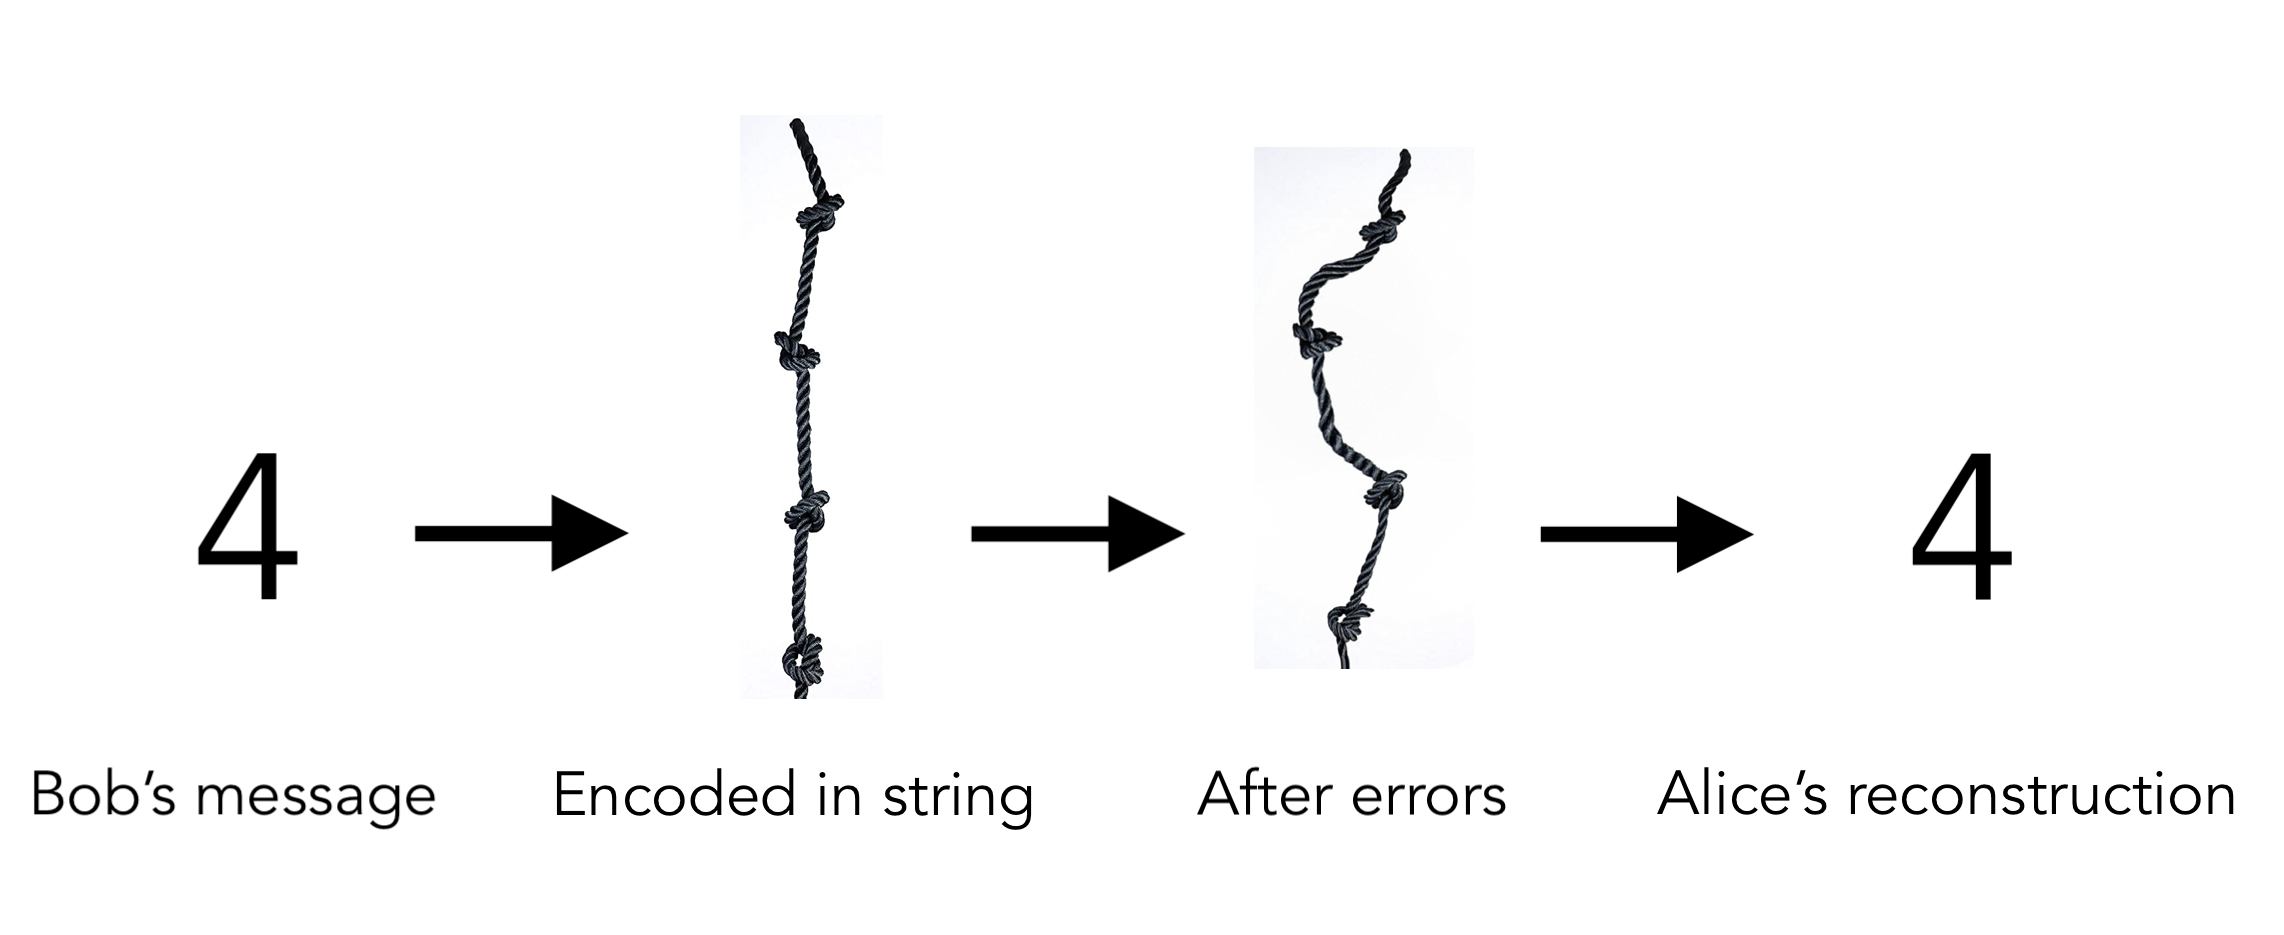
\includegraphics[scale=0.25]{rope-deformations}
\caption{A model of a (non-quantum) topological message}
\label{fig:rope-deformations}
\end{center}
\end{figure}

The answer is simple: Store the information in knots! By tying a certain number of simple knots in the string Alice can specify an integer that Bob can simply read off by counting (as in Figure \ref{fig:rope-deformations})! The beauty lies in the fact that while the string may be perturbed during the sending process, it would take a very specialized and unlikely error to untie the rope or to accidently re-tie an extra knot. This knotting number is a topological invariant (small perturbations don't change how many knots were tied), and so we can see intuitively that topological invariants are naturally error resistant.

The above situation is more than just a thought experiment: This is exactly the scheme that the ancient South American Incas used over 4000 years ago! The Incas stored all sorts of information in \textit{Quipus}, intricately knotted collections of fibered strings \cite{ascher1981code} as seen in Figure \ref{fig:quipu}. Storing information in knot invariants was also common practice in ancient Chinese, Tibetan, and Polynesian cultures \cite{day2021quipus}. In a sense, these are the earliest examples of topological computation.

\begin{figure}
\begin{center}
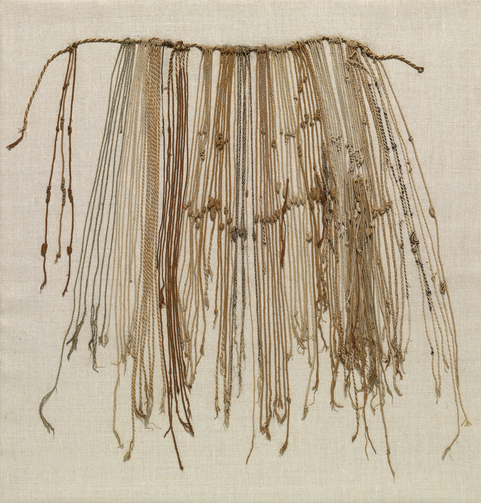
\includegraphics[scale=0.85]{quipu}
\caption{An Incan Quipu}
\label{fig:quipu}
\end{center}
\end{figure}

In TQC, information is still stored in knots. The main difference is that the strings being knotted are no longer physical pieces of twine, but \textit{trajectories of quasiparticles through spacetime}. For instance, suppose $X$ and $Z$ are two quasiparticles (we will elaborate more on this in later). Moving through space from time $t_0$ to $t_1$, the trajectories can look something like Figure \ref{fig:braiding}. Quantum interactions cause the knotting to yield real differences in physical states, and hence these knots can be used to store quantum information.

\begin{figure}
\begin{center}
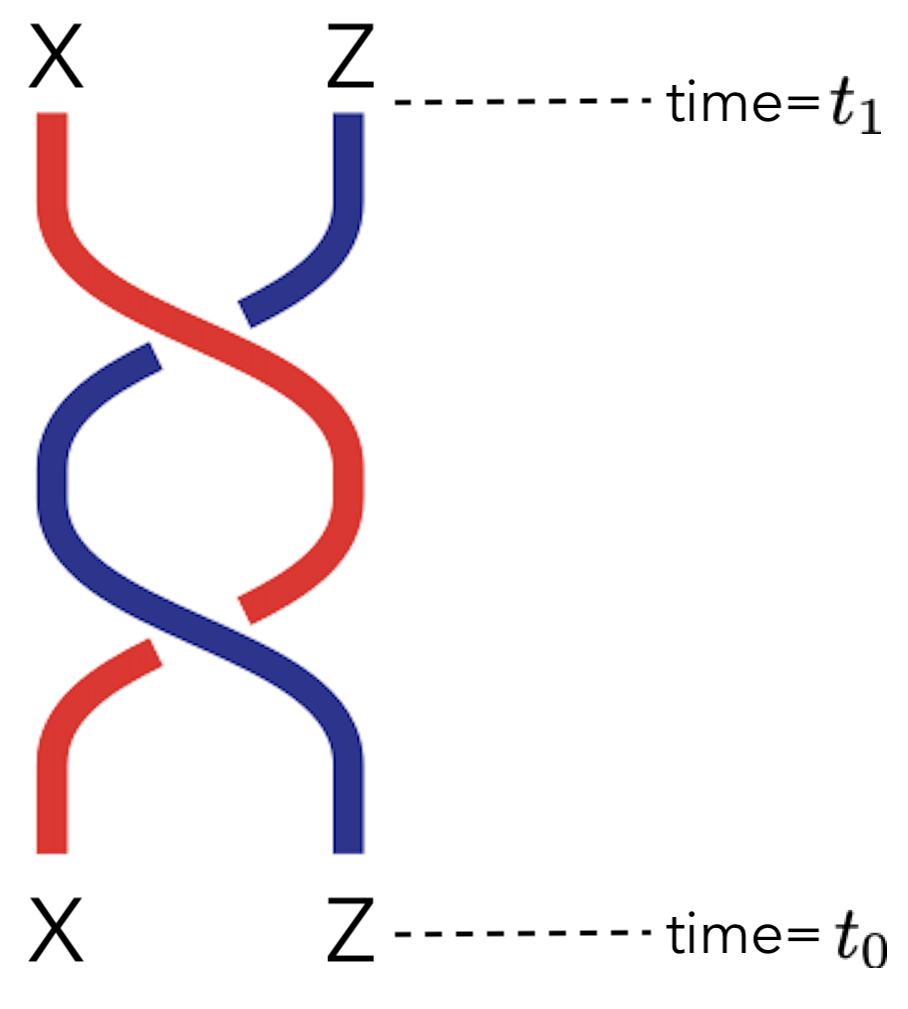
\includegraphics[scale=0.25]{braiding}
\caption{Braiding of quasiparticles in spacetime}
\label{fig:braiding}
\end{center}
\end{figure}

Notice that to make 3 dimensional spacetime, we modeled space as being 2 dimensional. While one might initially think this is a quirk of our human incapacity of visualizing 4 dimensional space, there is a deeper mathematical truth at play: There are no knots in 4 dimensional space. The extra dimension always gives the strands space to evade and move past each other without collision. In particular, for TQC to work we must have space be two dimensional. While this task seems initially impossible, phases of matter living entirely in a two dimensional subspace of our three dimensional world have been experimentally constructd\footnote{Of course, these are not \textit{literally} two dimensional. Motion in the third dimension is just so tightly constrained that $3$D models break down, and $2$D models start to work.}. Things that behave like particles in these 2 dimensional phases of matter are known as quasiparticles, and form non-trivial knots when braided.

The following is a rough description of how these 2 dimensional electron gasses are constructed. One begins by preparing a series of layers of graphene with a small gap in the middle. Upon subjecting the system to extremely cold temperatures and an extremely high magnetic field, the electrons in the graphene begin to move around. To balance the electric charge on both sides, all of the electrons move to the exact center of the setup. This resulting thin layer of electrons is a two dimensional electron gas. In such extreme conditions, all of the electrons will become highly entangled with each other, forming a quantum phase of matter \cite{yang2021experimental}. A diagram showing this process is found in Figure \ref{fig:spin-liquid}

\begin{figure}
\begin{center}
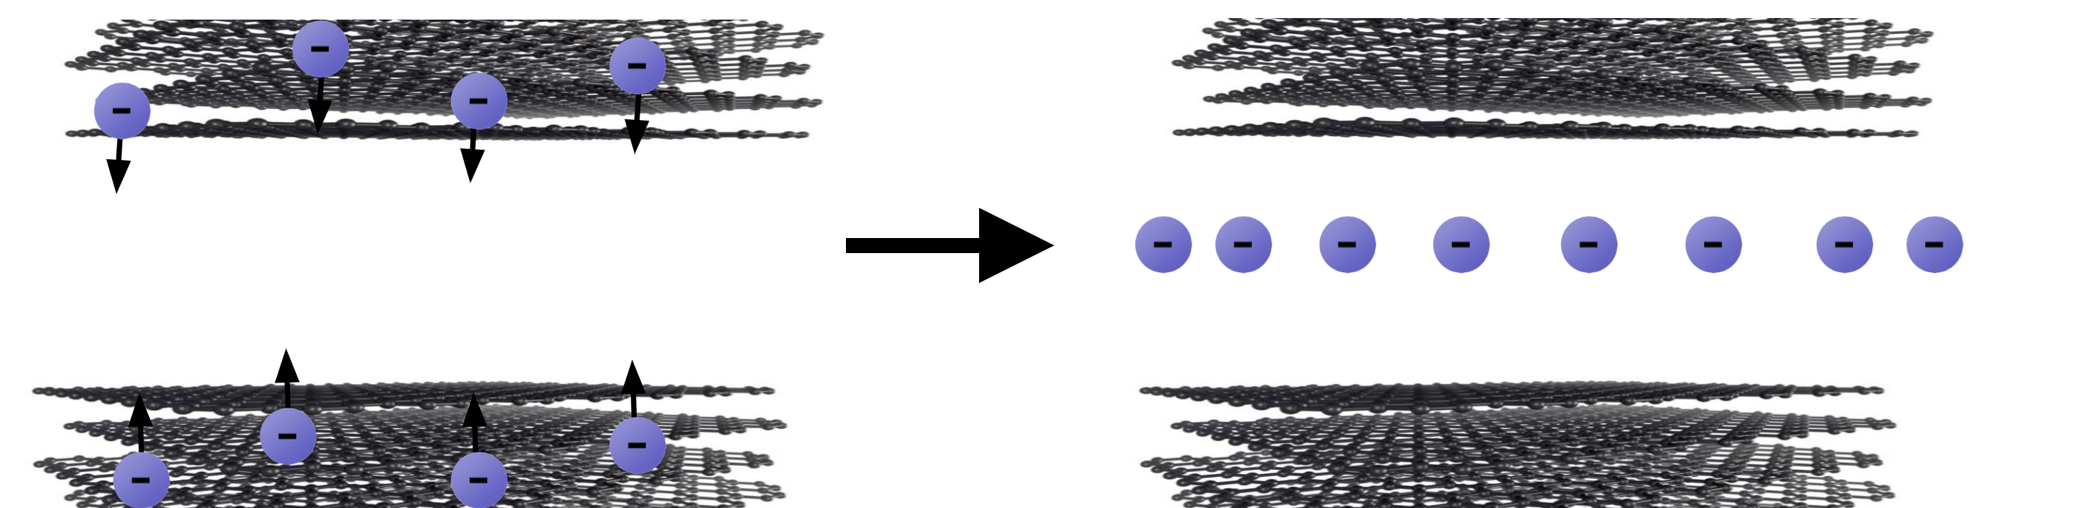
\includegraphics[scale=0.30]{spin-liquid}
\caption{The formation of an electron gas from graphene.}
\label{fig:spin-liquid}
\end{center}
\end{figure}

A key insight of Kitaev \cite{kitaev2003fault}, and one of the motivating pushes towards quantum computation, was that the topological properties of the 2 dimensional phase of matter will determine how the electrons entangled with each other. In other words, 2 dimensional sheets of electrons will form different quantum systems depending on their shape.

To understand this better, suppose that you have a 2 dimensional sphere of electrons. They will want to quantize, and align their spins together in the same direction. This amounts to choosing a unit tangent vector at each point on the sphere. However, there is no coherent way to do this. Every choice of tangent vectors will necessarily have some discontinuity or singularity: This is the content of the ``Hairy Ball Theorem".

If your sheet of electrons was on a donut, however, the situation is much different. There are several ways to coherently assign unit tangent vectors to each point; thus there are several ways for all of the electrons to quantize their spins together, as seen in Figure \ref{fig:hairy-ball}. This is aptly known as a \textit{spin liquid}. In mathematical language a ``donut" is called a torus, hence the name \textit{toric code}. The spin liquid associated with this procedure on a torus is called the ``$\ZZ_2$ spin liquid", and it is the physical realization of the toric code. We will spend the body of this manuscript describing the mathematics of the toric code in more detail. Note that generally when making such $\ZZ_2$ spin liquids in labs one does not make an actual torus; instead, one artificially simulates the boundary conditions of a torus in nanowires, for technical reasons \cite{albrecht2016exponential, mourik2012signatures}.

\begin{figure}
\begin{center}
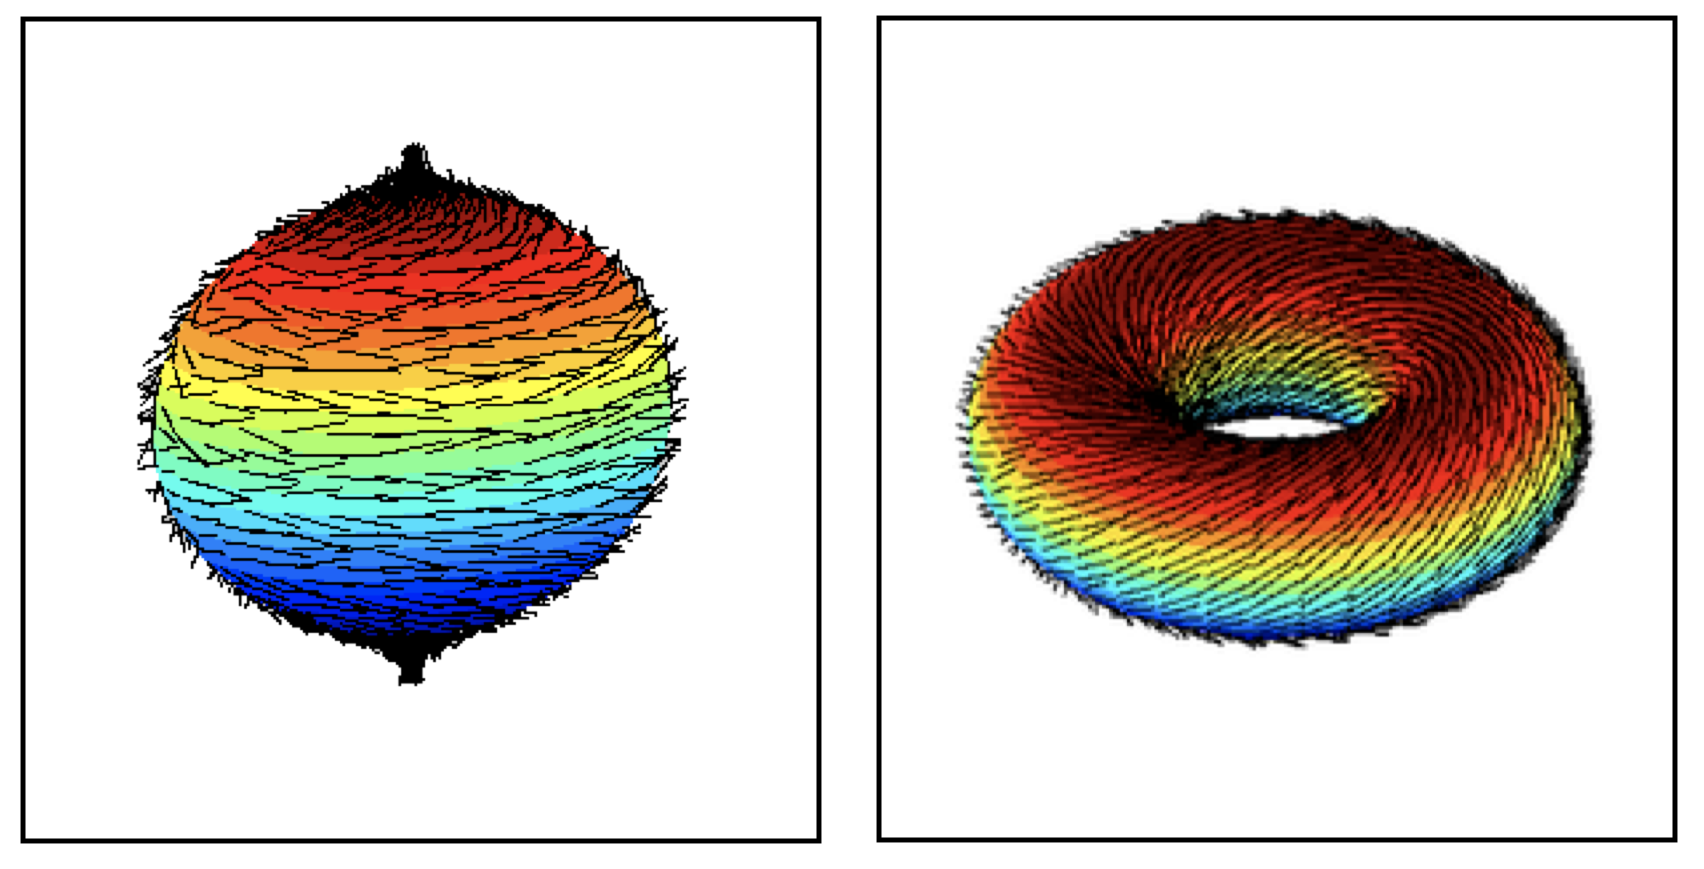
\includegraphics[scale=0.2]{Hairy-Ball-Diagram}
\caption{Assigning vector fields (spins) to a sphere, verses to a torus}
\label{fig:hairy-ball}
\end{center}
\end{figure}

We find it illustrative here to make an analogy with classical computing. Consider the following puzzle: Classical bits are stored in the magnetization of small regions on a hard disk. The magnetization of each atom is highly sensitive to thermal fluctuations. So why is it that classical computers seem so resistant to errors? The answer is that since all of the atoms are magnetized in the same direction, any one atom flipping will automatically be corrected back by the normalizing influence of the other atoms: magnets are naturally error resistant. It is exactly the same with these spin liquids that quantize together: Any one electron's spin decohering will immediately be corrected by the normalizing influence of all of its neighbors.

Before moving on to an in-depth treatment of the toric code, we offer a general description of the TQC process, in the style of the three points listed in the beginning of the introduction:

\begin{enumerate}
\item Information is stored in the ground states of topological quantum materials.
\item Ground states are acted on by braiding of quasiparticles, that is, by generating pairs of quasiparticles and knotting them in spacetime.
\item Measurements are performed by observing the topological properties of the resulting ground state.
\end{enumerate}

Here, \textit{ground state} refers to a state in the system with lowest possible energy. Note that in the previous description of spin liquids, all electrons having the same spin is a result of them being in the lowest energy state. An ``excited" electron with deviant spin will raise the energy of the system. In this way, quasiparticles can be interpreted as excitations of the topological quantum material. This motivates the fact that (topological) quantum computers must be exceptionally cold to function: Any extra energy will correspond to extra excitations, causing the computer to malfunction, since information is only stored in ground states.

The possibilities for topological quantum materials and TQC are extremely exciting, and we are eager to see where the field will go in the coming years.

\section{The Toric Code}
\label{The Toric Code}

Consider a torus. We will be imagining the torus as a whole as being a quantum system, corresponding physically to the quantum system one would observe when the torus is in the $\ZZ_2$ spin liquid topological quantum phase of matter. The \textit{code space} of the torus is the space of states on which we will be building our quantum computer, i.e., those states we will be using to store quantum information. In general Topological Quantum Computing (TQC) fashion, the code space of the toric code will be its ground states.

Our mathematical priorities are thus as follows: To define the quantum system, and to define a Hamiltonian operator on it. A Hamiltonian is an operator corresponding to the total energy of a quantum system. Namely, the eigenvalue of an eigenstate of the Hamiltonian corresponds to the total energy of that state. The code space will thus be the lowest eigenspace of the Hamiltonian.

\begin{figure}
\begin{center}
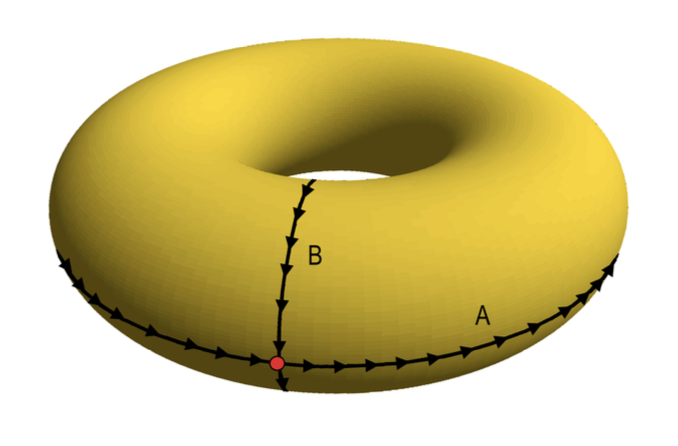
\includegraphics[scale=0.3]{torus}
\caption{Celluation of the torus, obtained by gluing opposite sides together.}
\label{fig:torus}
\end{center}
\end{figure}

Working with a continuous torus and the corresponding infinite dimensional vector spaces is cumbersome and unnecessary. Instead, we celluate the torus into an $n$ by $n$ square lattice with opposing sides identified, as in Figure \ref{fig:torus}. We will work with the understanding that the real physical system is the limit as $n\to\infty$. We define the quantum system associated with the $n$ by $n$ celluated torus to be the vector space

$$\Ncal=\bigotimes_{\substack{\text{edges of}\\\text{torus}}}\CC^2,$$

obtained by ``putting a qubit\footnote{A qubit is the quantum-computing term for ``two dimensional quantum system", i.e., $\CC^2$.}
on every edge". Here and throughout, \textit{vertices}, \textit{edges}, and \textit{faces}, when used as indexing sets, will refer to the set of \textit{vertices}, \textit{edges}, and \textit{faces} of our celluated torus. We will choose a canonical basis $\left\{\0,\1\right\}$ for $\CC^2$, reflecting our information theoretic intentions. To more forward with defining the Hamiltonian, we introduce the Pauli matrices

$$
\sigma_X=
\begin{pmatrix}
0 & 1\\
1 & 0
\end{pmatrix},\,\,
\sigma_Y=
\begin{pmatrix}
0 & -i\\
i & 0
\end{pmatrix},\,\,
\sigma_Z=
\begin{pmatrix}
-1 & 0\\
0 & 1
\end{pmatrix}.
$$

The Hamiltonian is defined by

$$H=-\sum_{\text{vertices } v}A_v-\sum_{\text{faces } p}B_p,$$

where

$$A_v=\bigotimes_{\substack{\text{edges}\\ \text{touching }v}}\sigma_Z,\,\, B_p=\bigotimes_{\substack{\text{edges}\\ \text{touching }p}}\sigma_X.$$

All of the power of the toric code comes from this highly non-obvious choice of Hamiltonian. The physical interpretation for this choice of Hamiltonian comes from gauge theory. Namely, the $U(1)$ Lattice Gauge Theory has two fields: The Compact Gauge Field and the Electric Field. Exponentiating the Compact Gauge Field we get the $\sigma_X$ operators, and exponentiating the Electric Field we get the $\sigma_Z$ operators. Thus, the $A_v$ contribute a ``Gauss' Law" term, and the $B_p$ contribute a ``Magnetic Field" term to the Hamiltonian \cite{oh2022rank}. While potentially physically illuminating, this discussion of gauge theory will have no influence on the rest of the mathematics presented in this manuscript, and does not need to be understood to appreciate the toric code.

Letting $I$ denote the identity matrix, the key facts about the $A_v$s and $B_p$s are summarized in the following proposition:

\begin{proposition}\label{AvBp}We have that

\begin{enumerate}[(i)]
\item $A_v^2=B_p^2=I$ for all $v,p$
\item All $A_v$s and $B_p$s have half eigenvalues $+1$ and half eigenvalues $-1$
\item All $A_v$s and $B_p$s commute
\item $\prod_{\text{vertices }v}A_v=I$ and $\prod_{\text{faces }p}B_p=I$
\end{enumerate}

\end{proposition}
\begin{proof}
$(i).$ Multiplying tensor product matrices corresponds to simply multiplying componentwise. Hence, this part  follows immediately from the relations $\sigma_X^2=\sigma_Z^2=I$.

$(ii).$ We define an isomorphism between the $+1$ eigenspace and $-1$ eigenspace of $A_v$. Namely, apply $\sigma_X$ to  an edge $e$ touching $v$. Since $\sigma_X\sigma_Z=-\sigma_Z\sigma_X$, the computation

$$A_v \left(\bigotimes_{\text{edge }e}\sigma_X\right)\ppsi = -A_v \left(\bigotimes_{\text{edge }e}\sigma_X\right)A_v\ppsi $$

show that a $+1$ eigenstate will be transformed into a $-1$ eigenstate, and a $-1$ eigenstate will be turned into $+1$ eigenstate. Thus, this defines an isomorphism between the desired eigenspaces. Applying $\sigma_Z$ instead of $\sigma_X$, we can define a similar isomorphism for $B_p$.

this will have the effect of turning a $+1$ eigenstate into a $-1$ eigenstate and vice-versa,

$(iii).$ All the $A_v$s commute with each other since $\sigma_Z$ commutes with itself, and all the $B_p$s commute with each other since $\sigma_X$ commutes with itself. What's left to check is that $A_vB_p=B_pA_v$. Notice that if $v$ is not touching the face $p$, none of the $\sigma_Z$s in the tensor product of $A_v$ will be in the same spots as any of the $\sigma_X$s as the tensor product for $B_p$. Hence, $A_v$ and $B_p$ commute in this case. If $v$ is touching $p$, then exactly two of the $\sigma_Z$s in the tensor product of $A_v$ will be in the same spots as $\sigma_X$s in the tensor product of $B_p$. Hence, pulling $B_v$ through $A_v$ corresponds to switching $\sigma_X$ and $\sigma_Z$. Since $\sigma_X\sigma_Z=-\sigma_Z\sigma_X$, this introduces an overall phase shift of $(-1)^2=1$. Hence, $A_vB_p=B_pA_v$ as desired!

$(iv).$ Applying $\prod_{\text{vertices } v}A_v$, is the same as applying $\sigma_Z$ to each vertex $2$ times, since each edge touches exactly $2$ vertices. Hence,

$$\prod_{\text{vertices } v}A_v=\bigotimes_{\text{edges}}\sigma^2_Z=\bigotimes_{\text{edges}}I=I.$$

Similarly, since every edge touches exactly $2$ faces, the fact that $\prod_{\text{faces } p}B_p=I$ follows from $\sigma^2_X=1$.
\end{proof}

Using the above facts about the $A_v$s and $B_p$s, we can describe the eigenspaces of $H$ well enough to compute their dimension:

\begin{proposition}\label{eigenspaces} All eigenvalues of $H$ are of the form $-2n^2+4q$, for an integer $q\leq n^2/2$. The $-2n^2+4q$ can be described as the space of states $\ppsi$ such that

$$\left|\left\{\left. v,p\right| A_v\ppsi =-1,\,\, B_p\ppsi=-1\right\}\right|=2q,$$

that is, the space of states with $2q$ excitations. There will always be an even number of $v$ such that $A_v\ppsi =-1$, as well as an even number of $p$ such that $B_p\ppsi=-1$. The dimension of of this eigenspace is

$$4\sum_{k=0}^{q}{n^2 \choose 2k} {n^2 \choose 2(q-k)}.$$

In particular, the code space of the toric code is 4 dimensional, and consists of those vectors $\ppsi$ such that $A_v\ppsi=B_p\ppsi=\ppsi$ for all $v,p$.
\end{proposition}
\begin{proof} To begin, we observe the following general fact from linear algebra. If $M$ and $N$ are commuting matrices and $\ppsi$ is an eigenvector for $N$ with eigenvalue $\lambda$, then

$$N(M\ppsi)=M(N\ppsi)=\lambda (M\ppsi).$$

Hence, $M$ respect the eigenspaces of $N$, and vice versa. This implies that the eigenspaces for $H$ will be simultaneous eigenspaces for all of the $A_v$s and $B_p$s, since all of the $A_v$s and $B_p$s commute by Proposition \ref{AvBp} (iii).

Suppose that $\ppsi$ is an eigenstate with

$$\left|\left\{\left. v,p\right| A_v\ppsi =-1,\,\, B_p\ppsi=-1\right\}\right|=q.$$

Then, we find that

\begin{align*}
H\ppsi&=(-\sum_{v}A_v-\sum_{p}B_p)\ppsi\\
&=\left(\sum_{\substack{v,p \\ -1\text{ eigenvalue}}}1-\sum_{\substack{v,p \\ 1\text{ eigenvalue}}}1\right)\ppsi\\
&=(q-(n^2-q))\\
&=-n^2+2q.
\end{align*}

Thus, to complete the initial description of the eigenstates, we must show that the number of $v$ such that $A_v\ppsi=-1$ and the number of $p$ such that $B_p\ppsi=-1$ is even. This follows from the computation that is this number where odd, then we would have by Proposition \ref{AvBp} (iv) that

$$\ppsi = \left(\prod_{v}A_v\right) \ppsi = -\ppsi,$$

which is a contradiction since we are supposing that $\ppsi\neq 0$. The exact same argument applies to the $B_p$. We now compute the dimensions of the eigenspaces. Let $D$ denote the dimension of the group space. We show that given any even sized sets $\bold{v}, \bold{p}$ of vertices and faces respectively, the space

$$\Ncal_{\bold{v},\bold{p}}=\{\left.\ppsi\right| \left(A_v\ppsi=-1\iff v\in \bold{v}\right),\,\, \left(B_p\ppsi=-1\iff p\in\bold{p}\right) \}$$

is $D$ dimensional. We proceed by induction on $|\bold{v}+\bold{p}|$. If $|\bold{v}+\bold{p}|=0$, then this is the definition of $D$. Without loss of generality, suppose $|\bold{v}|\geq 2$. If $|\bold{p}|\geq 2$, we apply the same arguement with verticies replaced by faces. Choose two verticies $v_0,v_1\in \bold{v}$. Choose a path $\gamma$ along the edges of the torus that connect $v_0$ and $v_1$. We show that $\bigotimes_{\text{edges in }\gamma}\sigma_X$ gives an isomorphism between $\Ncal_{\bold{v},\bold{p}}$ and $\Ncal_{\bold{v}-\{v_0,v_1\},\{p\}}$. Namely it is clear from $\sigma_X^2=\sigma_X$, so this map is its own inverse, so it is sufficient to show that the image is in the desired space. To prove this, we observe that $\bigotimes_{\text{edges in }\gamma}\sigma_X$ commutes with all the $B_p$s, and commutes with all of the $A_v$s at verticies that $\gamma$ passes through an even number of times. The only verticies that $\gamma$ passes through an odd number of times are its endpoints (by definition), and hence $A_v$ has exactly the effect of flipping the eigenvalues at $A_{v_0}$ and $A_{v_1}$. Thus, the image of a point in $\Ncal_{\bold{v},\bold{p}}$ is in $\Ncal_{\bold{v}-\{v_0,v_1\},\bold{p}}$, as desired.

Combining, we find that the $-2n^2+2q'$ eigenstate can be decomposed as direct sums of $\Ncal_{\bold{v},\bold{p}}$, where $\bold{v}$ and $\bold{p}$ range over even sized sets with $|\bold{v}+\bold{p}|=q'$. In particular, $q'=2q$ must be even. The dimension of this space is equal to $D$ times the number of way of choosing the sets $\bold{v}$ and $\bold{q}$, i.e.,

$$D\sum_{k=0}^{q}{n^2 \choose 2k}{n^2 \choose 2(q-k)}.$$

The total dimension of eigenspaces of $H$ can be computed as

\begin{align*}
D\sum_{q=0}^{2n^2}\sum_{k=0}^{q}{n^2 \choose 2k}{n^2 \choose 2(q-k)}&=D\left(\sum_{q=0}^{2n^2}{n^2 \choose 2k_0}\right)\\
&=D\cdot \left(2^{n^2-1}\right)^2=D\cdot 2^{2n^2-2}.
\end{align*}

The Hamiltonian is a symmetric matrix with real coefficients, since it is the tensor product of such matrices. It is a standard fact from linear algebra that such matrices can be diagonalized, and hence the total dimension $H$ is equal to the dimension of $\Ncal=\bigotimes_{\text{edges}}\CC^2$. Seeing as there are $2n^2$ edges this space is $2^{2n^2}$ dimensional, and hence we must have $D=2^2=4$.
\end{proof}

The fact that the code space is four dimensional can be motivated as follows. By Proposition \label{AvBp} (ii), being in the $+1$ eigenspace for each $A_v$ and $B_p$ will impose a condition that decreases the dimension of your space by $1/2$. Since $\Ncal$ is $2^{2n^2}$ dimensional, imposing all $n^2$ of these conditions decreases the code space to $1$ dimension. However, the fact that $\prod_{\text{vertices }v}A_v=I$ and $\prod_{\text{faces }p}B_p=1$  from Proposition \label{AvBp} (iv) shows that two of these conditions imposed were redundant, brining the code space dimension back up to $2^2=4$ dimensions.

To describe the generators of the codespace explicitly we will need to use the basics of homology theory with $\ZZ_2$ coefficients, where $\ZZ_2=\{0,1\}$ is the additive group modulo $2$. For those unfamiliar, a brief introduction is included in Appendix \ref{Homology}.

\begin{figure}
\begin{center}
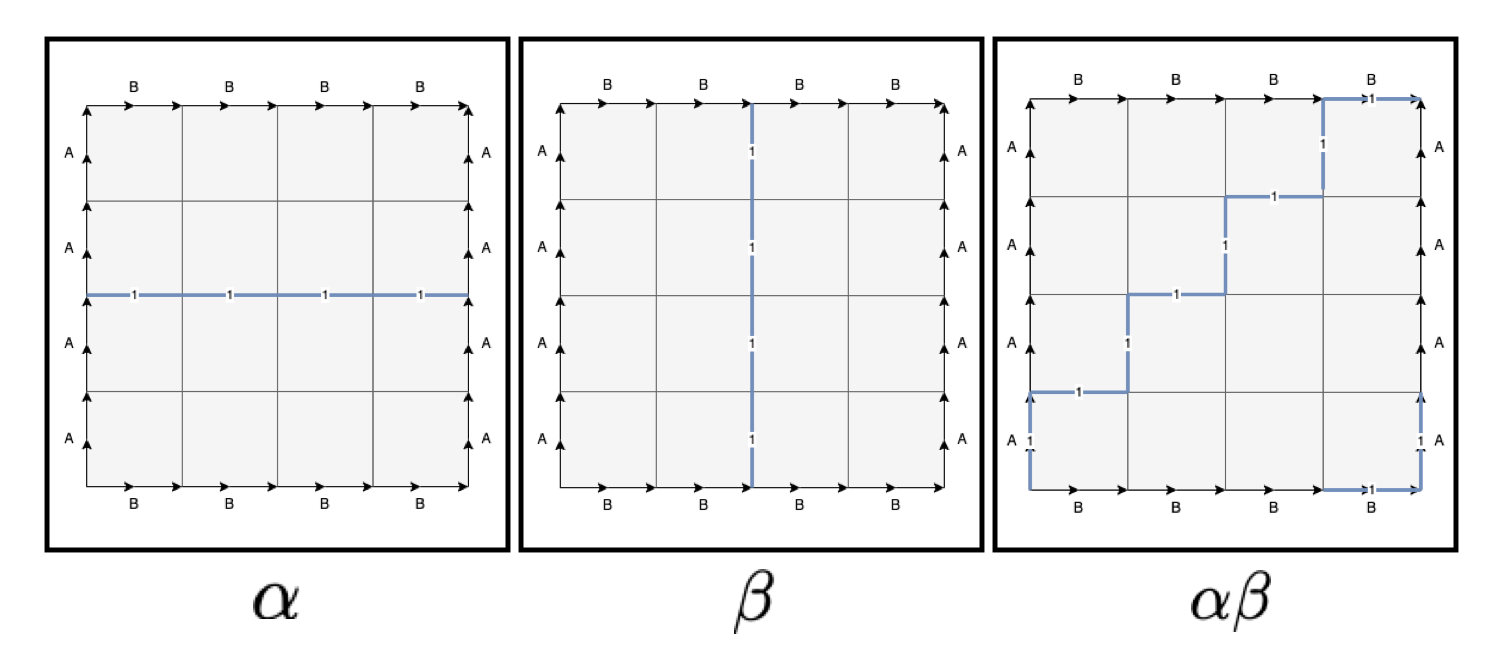
\includegraphics[scale=0.35]{homology-classes}
\caption{The three non-trivial homology classes of a torus}
\label{fig:homology}
\end{center}
\end{figure}


A pure state on $\Ncal$ is specified by a pure state on each qubit, namely, a choice of $\0$ and $\1$ for each edge. This is exactly the data to specify a $\ZZ_2$-chain. Given a $\ZZ_2$-chain $\gamma$, we write $\left|\gamma\right>$ for the associated pure state. Given any $\gamma,\gamma'$, we write $\gamma\sim \gamma'$ to mean that $\gamma$ and $\gamma'$ are homologous. The following elucidates the meaning of the codespace of the toric code:

\begin{proposition}\label{basis} Let $\bold{0},\alpha,\beta,$ and $\alpha\beta$ be the four $\ZZ_2$ homology classes on the torus, as in Figure \ref{fig:homology}. Choose $\bold{0}_0$, $\alpha_0$, $\beta_0$, and $(\alpha\beta)_0$ respectively to be representatives. Then, letting $\gamma$ run over all $\ZZ_2$-cycles, we have that

\begin{align*}
\nullclass &= \frac{1}{\sqrt{2^{n^2-1}}}\sum_{\gamma\sim \bold{0}_0}\left|\gamma\right>,\,\, \alphaclass=\frac{1}{\sqrt{2^{n^2-1}}}\sum_{\gamma\sim \alpha_0}\left|\gamma\right>,\\
\betaclass &= \frac{1}{\sqrt{2^{n^2-1}}}\sum_{\gamma\sim \beta_0}\left|\gamma\right>,\,\, \alphabetaclass=\frac{1}{\sqrt{2^{n^2-1}}}\sum_{\gamma\sim (\alpha\beta)_0}\left|\gamma\right>,
\end{align*}

are all normalized eigenstates of that Hamiltonian $H$, and serve as a canonical orthonormal basis of the codespace.
\end{proposition}
\begin{proof} Choose $\omega\in H_1(T;\ZZ_2)$. To show that $\left|\omega\right>$ is in the codespace, we observe that it is in the $+1$ eigenspace of every $A_v$ and $B_p$. Since $\sigma_Z$ sends $\0$ to $\0$ and $\1$ to $-\1$, $A_v$ has the effect of sending a pure state $\left|\gamma\right>$ to $\pm\left|\gamma\right>$, depending on whether $\gamma$ has an odd or even count of edges touching the vertex $v$. In particular, because $\gamma$ is running over cycles, we have that each $\left|\gamma\right>$ is in the $+1$ eigenspace of all the $A_v$, and hence the same applies to $\left|\omega\right>$.

For $B_p$s, we observe that applying $B_p$ to a pure state $\left|\gamma\right>$ has the effect of flipping all of the qubits around the face $p$. By definition of being $\ZZ_2$ homologous, $B_p$ maps the space of all cycles homologous to $\left|\omega\right>$ back into the space of all cycles homologous to $\left|\omega\right>$. In particular, $\left|\omega\right>$ is in the $+1$ eigenspace of $B_p$ for every $p$.

To show that $\left|\omega\right>$ is normalized, we observe that there are exactly that there are exactly $2^{n^2-1}$ cycles homologous to $\omega$. This is proved as follows. Starting with a fixed representative $\omega_0$ of $\omega$, cycles homologous to $\omega$ correspond to flipping qubits around the edges, i.e., applying $B_p$s at faces. Since there are $n^2$ faces, this gives $2^{n^2}$ cycles. This overcounts the space of cycles homologous to $\omega$ by a factor of $2$, since $\prod_{\text{faces }p}B_p=I$ by Proposition \ref{AvBp} (iv). The fact that the codespace is 4 dimensional says that this is the \textit{only} relation between the $B_p$s. Hence, there are $2^{n^2-1}$ cycles.

To show that these states are mutually orthogonal, we observe simply that no cycle can be homologous to two of the $\{\bold{0},\alpha,\beta,\alpha\beta\}$, hence $\left\{\nullclass,\alphaclass,\betaclass,\alphabetaclass\right\}$ have disjoint support, hence they are orthogonal.
\end{proof}

Letting $T$ denote the torus, the above shows that we can view the codespace of the toric code as a physical realization of the vector space $\CC[H_1(T;\ZZ_2)]$. Here, $\CC[A]$ for some set $A$ denotes the vector space generated by $A$, i.e., the unique complex vector space which has a basis given by $A$. Quantum physics gives the physical analogue of the abstract mathematical notation of an equivalence class, namely, an equivalence class is realized as the superposition over all possible representatives. This can be compared with the path integral formulation of quantum mechanics, where one integrates over all possible paths between two points.

We now give \textit{quasiparticle} interpretation of the toric code. A quasiparticle is an excitation in the toric code. Namely, given an eigenstate $\ppsi$, we say that there is a quasiparticle at a vertex $v$ if $A_v\ppsi=-\ppsi$, and get a face $p$ we say that there is a quasiparticle at $p$ if $B_p\ppsi=-\ppsi$.

Let $\ppsi$ be an eigenstate, and let $v_0,v_1$ be adjacent vertices connected by an edge $e$. Suppose that there is a quasiparticle at $v_0$, and that there is not a quasiparticle at $v_1$. Let $\left| \psi'\right>$ be the state obtained by applying $\sigma_X$ to the edge $e$. We observe that

$$A_{v_0}\left| \psi'\right> = A_{v_0}\left(\bigotimes_{\text{edge }e}\sigma_X\right)\ppsi=-A_{v_0}\ppsi=\ppsi,$$

$$A_{v_1}\left| \psi'\right> = A_{v_1}\left(\bigotimes_{\text{edge }e}\sigma_X\right)\ppsi=-A_{v_1}\ppsi=-\ppsi,$$

where we used the key fact that $\sigma_X\sigma_Z=-\sigma_Z\sigma_X$. Additionally, $A_{v}\left|\psi'\right>=A_{v}\ppsi$ for $v\neq v_0,v_1$, since applying $\sigma_X$ to $e$ only affects the verticies $v_0$ and $v_1$. We can interpret this computation as saying the following: Applying $\sigma_X$ has the effect of \textit{moving the quasiparticle along e}, from $v_0$ to $v_1$. Applying longer chains of $\sigma_X$s, we see in general that applying $\sigma_X$ corresponds to moving quasiparticles at verticies along the edges. If neither $v_0$ nor $v_1$ had quasiparticles, then again tensoring with $\sigma_X$ at $e$ would have the effect of flipping the eigenvalues at $v_0$ and $v_1$, i.e., the effect of \textit{creating quasiparticles at the endpoints of e}, at $v_0$ and $v_1$. If both $v_1$ and $v_1$ has quasiparticles, then tensoring with $\sigma_X$ at $e$ would have the effect of \textit{anhilating quasiparticles at the endpoints of e}.

In summary, the quasiparticles at edges are their own antiparticle. Creating particle/antiparticle pairs, moving the quasiparticles, and annihilating particle/antiparticle pairs all are mathematically realized by the simple operation of tensoring edges with $\sigma_X$.

Similarly, we can describe the quasiparticles sitting at faces, corresponding to faces with an excitation $B_p\ppsi=-\ppsi$. Tensoring with $\sigma_X$ has no effect on these quasiparticles, since tensoring with $\sigma_X$ at any edge commutes with all the $B_p$: $\sigma_X$ commutes with itself. However, it is now tensoring with $\sigma_Z$ that causes the motion of particles. Given faces $p_0,p_1$ with common edge $e$, tensoring with $\sigma_Z$ at $e$ has the effect of moving a quasiparticle from $p_0$ to $p_1$ if exactly one of the faces had a quasiparticle, has the effect of creating a particle/antiparticle pair if neither of the faces has quasiparticles, and has the effect of annihilating a particle/antiparticle pair if both faces have quasiparticles.

Summarizing, we find that the toric code naturally have two types of quasiparticles, an $X$-type that lives on vertices which moves by tensoring by $\sigma_X$, and a $Z$-type that lives in faces and moves by tensoring with $\sigma_Z$. This allows us to mathematically implement a topological quantum computer. Namely:

\begin{enumerate}
\item Quantum information is stored in the ground state of the toric code, i.e., the lowest eigenvalue eigenspace of the Hamiltonian.
\item Ground states are acted on by generating and manipulating quasiparticles, moving them around the torus, and annihilating them. Mathematically, this is realized by repeatedly tensoring with $\sigma_X$ and $\sigma_Z$ along edges, until one returns to a ground state.
\item Quantum information is measured by observing the ground state with respect to the canonical orthonormal basis of the codespace, given in Proposition \ref{basis}
\end{enumerate}


As an example, we implement the ``$\text{NOT}_\alpha$" gate, which flips the input state depending on whether it has an $\alpha$ component, namely

\begin{align*}
&\nullclass \mapsto \alphaclass,\,\,  \betaclass \mapsto \alphabetaclass \\
&\alphaclass \mapsto \nullclass,\,\, \alphabetaclass \mapsto \betaclass.
\end{align*}

\begin{figure}
\begin{center}
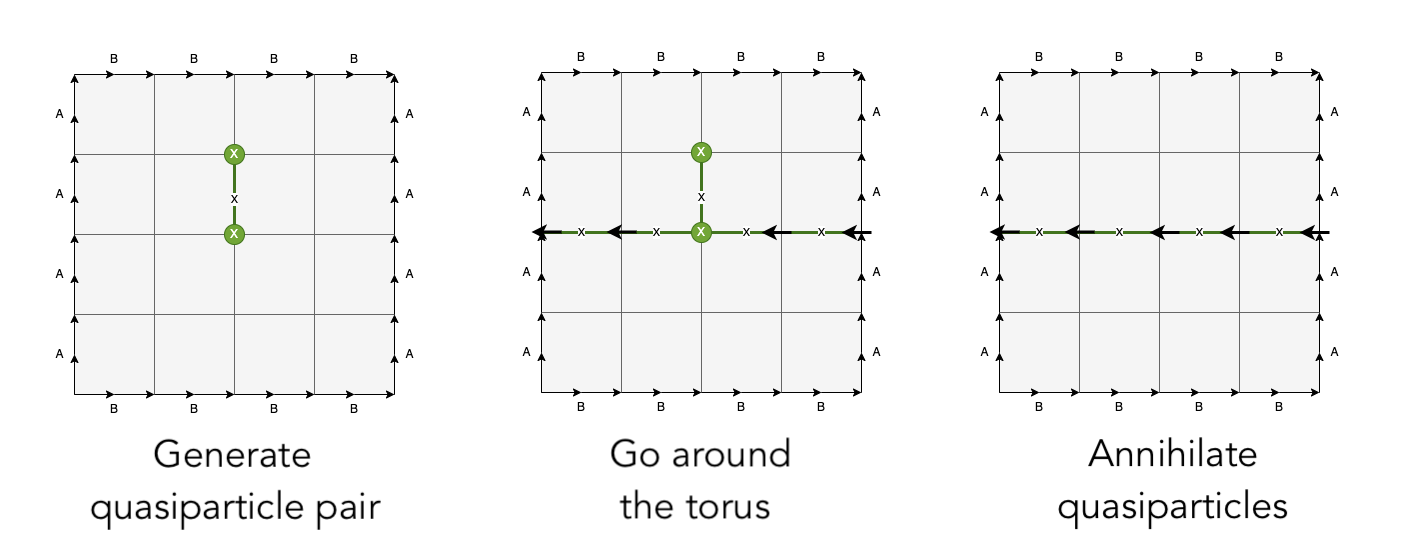
\includegraphics[scale=0.45]{not-alpha-gate}
\caption{Topological quantum process implementing the $\text{NOT}_{\alpha}$ gate}
\label{fig:not-alpha-gate}
\end{center}
\end{figure}

A diagram visualizing the process described in the following proposition is shown in Figure \ref{fig:not-alpha-gate}.

\begin{proposition} The following computation has the effect of performing the $\text{NOT}_{\alpha}$ gate. First, generate a particle/antiparticle pair of $X$-type particles. Then, move one of the particles around the torus via a path homologous to $\alpha$. Finally, fuse your two adjacent $X$-type particles together.
\end{proposition}
\begin{proof} Let $v_0$ and $v_1$ be adjacent vertices. Let $\alpha_0$ be a cycle homologous to $\alpha$ going from $v_1$ to itself. The process described in the statement of the proposition can be reworded as saying the following. First, we create a particle pair at $v_0$ and $v_1$, i.e., we tensor with $\sigma_X$ at the edge connecting $v_0$ and $v_1$. Then we move $v_1$ along $\alpha_0$, i.e., we tensor with $\sigma_X$ along the edges in $\alpha_0$. Then, we fuse the $X$-type quasiparticles at $v_0$ and $v_1$ back together, i.e., we tensor along the edge connecting $v_0$ and $v_1$ again. Since $\sigma_X^2=1$, this whole process can be described mathematically as

$$\bigotimes_{\text{edges in }\alpha_0}\sigma_X.$$

Seeing as $\sigma_X$s corresponds to flipping $\0$s to $\1$s in pure states, this process has the effect of flipping all of the qubits along $\alpha_0$. On the level of cycles, this means that we take $\left|\gamma\right>$ to $\left|\gamma+\alpha_0\right>$, where addition is in the group of cycles. Seeing as adding a cycle homologous to $\alpha$ to a cycle homologous to $\omega$ results in a cycle homologous to $\omega+\alpha$ we find thus that this process has the effect of sending $\left|\omega\right>$ to $\left|\omega+\alpha\right>$. Seeing as $\alpha+\alpha=0$ in $H_1(T;\ZZ_2)$, this process is exactly the $\text{NOT}_{\alpha}$ gate.
\end{proof}

Similarly, we can implement the $``(-1)_{\alpha}"$ gate, which flips the input state depending on whether it has an $\alpha$ component, namely

\begin{align*}
&\nullclass \mapsto \nullclass,\,\,  \betaclass \mapsto \betaclass \\
&\alphaclass \mapsto -\alphaclass,\,\, \alphabetaclass \mapsto -\alphabetaclass.
\end{align*}

\begin{proposition}\label{Xparticle} The following computation has the effect of performing the $\text{(-1)}_{\alpha}$ gate. First, generate a particle/antiparticle pair of $Z$-type particles. Then, move one of the particles around the torus via a path homologous to $\beta$. Finally, fuse your two adjacent $Z$-type particles together.
\end{proposition}
\begin{proof} Let $p_0$ and $p_1$ be adjacent faces. Let $\beta_0$ be a cycle homologous to $\beta$ going from $p_1$ to itself. Note that since $Z$-type particles live on faces, $\beta_0$ does not consist of a series of edges. Instead, it is a path going through the centers of faces. We take $\widehat{\beta}_0$ to be the set of edges that $\beta_0$ passes through. Tensoring with $\sigma_Z$ along $\widehat{\beta}_0$ corresponds to motion of a particle from $p_1$ along $\beta_0$ back to itself.

\begin{figure}
\begin{center}
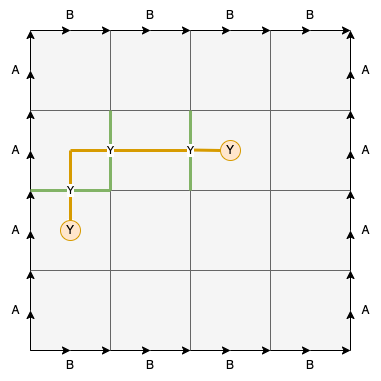
\includegraphics[scale=0.30]{dual-celluation}
\caption{Sample trajectory along dual celluation of torus}
\label{fig:dual-celluation}
\end{center}
\end{figure}

These cycles that go through faces of the torus are called \textit{dual cycles}, and are standard practice in the theory of homology. Namely, they are cycles in the dual celluation, as seen in Figure \ref{fig:dual-celluation}. Whereas the edges associated with a normal cycle satisfy the property `every vertex touches an even number of $1$s', the edges associated with a cycle in the dual celluation satisfy the dual condition `every face touches an even number of $1$s'.

As before, we find that the whole process can be described mathematically as

$$\bigotimes_{\text{edges in }\widehat{\beta}_0}\sigma_Z.$$

The matrix $\sigma_Z$ acts on pure states by sending $\0$ to itself, and $\1$ to $-\1$. Thus, this process has the effect of introducing a $-1$ global phase shift for every $1$ in states along $\widehat{\beta}_0$. Thus, when acting on a pure state $\gamma$, the definition of $\widehat{\beta}_0$ shows that this process has the effect of introduce a phase shift of $-1$ to the power of the number of intersection between $\gamma$ and $\widehat{\beta}_0$.

It is a well known fact that this signed intersection number ($-1$ to the power of the number of intersections) is an invariant in $\ZZ_2$ homology. To see this, observe that changing representatives of a homology class correspond to flipping qubits around a face. By the `dual cycle' condition, this flipped face will touch an even number of elements in the dual cycle. Hence, the intersection number will change by an even amount, leaving $-1$ to the power of that number invariant.

In particular, $\bold{0}$ doesn't intersect $\beta$, $\beta$ doesn't intersect $\beta$ (representatives can be chosen to be parallel), $\alpha$ intersects $\beta$ (horizontal loops and vertical loops meet at exactly one point), and $\alpha\beta$ intersects $\beta$. Thus, this process has the effect of adding a $-1$ phase shift to those states which include an `$\alpha$', as desired.
\end{proof}

Sadly for the toric codes, these are essentially the only gates that can be implemented. No matter how one moves around particles, there is not enough complexity in the system to generate interesting gates. We formalize this by writing out the \textit{group of gates} of the toric codes. We can think of quantum gates on a system as forming a group, where the group law is given by the composition of gates, and every element has an inverse since unitary matrices are invertible. For the toric codes, we have the following:

\begin{proposition}\label{Yparticle} There are exactly 8 possible computations in the toric codes. The group of gates is (non canonically) isomorphic to the Pauli group, i.e., the group whose objects are

$$\{\pm I, \pm iI, \pm \sigma_X, \pm i \sigma_X, \pm \sigma_Y, \pm i\sigma_Y, \pm \sigma_Z, \pm i \sigma_Z\}$$

and whose group operation is given by matrix multiplication. A minimal generating set is given by $\{\text{NOT}_{\alpha},\text{NOT}_{\beta},(-1)_{\alpha}\}$.
\end{proposition}
\begin{proof} To begin, we define $\text{NOT}_{\beta},\text{NOT}_{\alpha\beta},(-1)_{\beta},$ and $(-1)_{\alpha\beta}$ in complete analogy to how we define $\text{NOT}_{\alpha}$ and $(-1)_{\alpha}$. Namely, $\text{NOT}_{\beta}$ flips whether or not a state has a `$\beta$' in it, and $\text{NOT}_{\alpha\beta}$ flips whether or not a state has an `$\alpha\beta$' in it, i.e.,

\begin{align*}
&\nullclass \mapsto \alphabetaclass,\,\,  \betaclass \mapsto \alphaclass \\
&\alphaclass \mapsto \betaclass,\,\, \alphabetaclass \mapsto \nullclass.
\end{align*}

The relation $\sigma_X\sigma_Z=-\sigma_Z\sigma_X$ implies that we can switch the order of operations between first applying all our $\sigma_X$s and then applying all our $\sigma_Z$s, up to an operator-wise phase shift $-1$. Any process of creating and annihilating $X$-type quasiparticles can be modeled in sequence as repeatedly creating particles, moving them around a loop, then annihilating them. Following the proof of Proposition \ref{Xparticle}, this is the same as repeatedly applying $\text{NOT}_{\omega}$ gates, for homology classes $\omega$. Similarly, the processes on $Z$-type particles will be compositions of $(-1)_{\omega}$ gates.

Hence, we now have a full set of generators for our gate group: $\{\pm I, \text{NOT}_{\omega}, (-1)_{\omega}\}$, where $\omega$ runs over homology classes. The relations $\text{NOT}_{\alpha}\text{NOT}_{\beta}=\text{NOT}_{\alpha\beta}$ and $(-1)_{\alpha}(-1)_{\beta}=(-1)_{\alpha\beta}$ allow one to reduce the generating set further. The relations

$$\text{NOT}_{\alpha}(-1)_{\alpha}\text{NOT}_{\alpha}=(-1)_{\beta}$$

and

$$(-1)_{\alpha}\text{NOT}_{\alpha}(-1)_{\alpha}=-I$$

reduce the generating set to $\{\text{NOT}_{\alpha},\text{NOT}_{\beta},(-1)_{\alpha}\}$. Verifying simple relations gates, it is simple to see that the gate group is isomorphic to the Pauli group, as desired.


\end{proof}


Before moving on to the next section, we make a few final remarks about the behavior of quasiparticles on the toric codes. Namely, we observe the following. Consider the full vector space $\Ncal$, and adjacent two adjacent $X$-type and $Z$-type quasiparticles. Consider the simple braiding of these particles around each other, as in Figure \ref{fig:braiding}. A line going under another corresponds to the particle having passed through that space first, before the other particle. This braiding can be obtained by first performing a twist halfway around the circle by $X$, then a twist all the way around the circle by $Z$, then finally moving the second half of the circle by $X$. This process corresponds to a transformation $\Ncal\to \Ncal$ (i.e. tensoring with the appropriate $\sigma_X$s and $\sigma_Z$s). The observation is that this transformation is \textit{not} the identity on the codespace. Namely, since $\sigma_Z\sigma_X=-\sigma_X\sigma_Z$, this operation corresponds to a global phase shift of $-1$ on the system.

Thus, the braiding of $X$ type and $Z$ type particles corresponds to a phase shift of $-1$. This is in contrast to braiding two identical $X$ type or $Z$ type particles, which corresponds to the identity since $\sigma_X$ and $\sigma_Z$ commute with themselves. All particles in the standard model of physics are \textit{fermions}, which give a phase shift of $-1$ when you braid them with themselves, or \textit{bosons}, which act by the identity when you braid them with themselves. Seeing as $X$ type and $Z$ type particles in the toric code braid by the identity with themselves, one would expect them to be bosons. However, bosons always braid by the identity with each other and hence the $-1$ phase shift from braiding $X$ and $Z$ type particles should be impossible. The conclusion is that these really are \textit{quasi}particles, which behave much differently than particles in the standard model. Quasiparticles with simultaneously non-bosonic and non-fermionic braiding rules are known as \textit{anyons}. All interesting particles in topological quantum phases of matter will be anyons.

In the case of the toric code, the braiding will always be trivial or give a global phase shift (i.e. -1). We call anyons \textit{non-abelian} if they can braid in such a way to create transformations that are not phase shifts. To  create interesting quantum gates, these sort of non-phase shift braidings are what we need. The search for a topological quantum computer is essentially the search for experimentally-sound easy-to-braid non-abelian anyons.

$\newline\newline$

\large \textbf{Exercises}:\normalsize

\begin{enumerate}[\thesection .1.]
\item For edges $v$ and faces $p$, define

$$A_v'=\bigotimes_{\substack{\text{edges} \\ \text{touching }v}}\sigma_X,\,\, B_p'=\bigotimes_{\substack{\text{edges} \\ \text{touching }p}}\sigma_Z,$$

$$H'=-\sum_{\text{vertices }v}A_v'-\sum_{\text{faces }p}B_p'.$$

Let $M=\frac{1}{\sqrt{2}}
\begin{pmatrix}
1 & 1 \\
1 & -1
\end{pmatrix}$ be the Hadamard matrix. Using the relations

$$\sigma_X=M\sigma_ZM^{-1},\,\, \sigma_{Z}=M\sigma_X M^{-1},$$

show that $H$ and $H'$ are similar, in the sense that $H'=MHM^{-1}$. Use this to conclude that all basis independent properties of the toric code are formally symmetric by replacing $X$ with $Z$. In particular, the codespace (lowest eigenspace) of $H'$ is 4 dimensional, and the gate group of $H'$.


\item Show that eigenvectors of the Hamiltonian are equally likely to give $0$ or $1$ when measured at every qubit. This implies that the eigenvectors of the Hamiltonian are \textit{maximally entangled}, which is a more general phenomenon in TQC. (HINT: Prove this for ground states first, then lift to general eigenstates using an induction argument along the lines of the proof of Proposition \ref{eigenspaces})

\item Let $\Ncal_{n}$ denote the vector space associated to the $n$ by $n$ grid on the torus. Let

$$\tilde{H}_n=H_n+(2n^2)I,$$

so that the ground states have eigenvalue $0$. This is more physically realistic, since systems cannot have negative energy. When $n$ divides $m$, we have a natural map

$$\Ncal_{n}\hookrightarrow{}\Ncal_{m}$$

defined by [WORK: What is the correct definition?]. Show that this map is linear and injective, and hence that $\Ncal_{n}$ can be realized as a sub vector space of $\Ncal_{m}$. Show that $\tilde{H}_{m}$ restricted to $\Ncal_{n}$ is equal to $\tilde{H}_n$. Show that the map $\Ncal_{n}\hookrightarrow{}\Ncal_{m}$ is norm-preserving, in the sense that if $\left|\chi\right>,\left|\psi\right>$ are states on $\Ncal_{n}$, the inner product $\left<\chi | \psi \right>$ is independent of whether or not it was computed in $\Ncal_{n}$ or $\Ncal_{m}$. Define

$$\Ncal_{\infty}=\bigcup_{n=3}^{\infty}\Ncal_{n},$$

and define $\tilde{H}_{\infty}$ to be the operator on $\Ncal_{\infty}$ which acts on vectors in $\Ncal_{n}$ by $\tilde{H}_n$. Show that these are well defined objects, that $\Ncal_{\infty}$ is naturally a Hilbert space. It is in this sense that we can speak of a limiting continuous model formed by the discrete grid celluations\footnote{Note that objects in $\Ncal_{\infty}$ themselves aren't continuous paths; they are just discrete cycles in $\Ncal_n$ for some $n$. This is not an issue, since the \textit{simplicial approximation theorem} says that every continuous phenomenon can be modeled discreetly in a fine enough celluation.}.
\end{enumerate}

\section{Topological Quantum Field Theories}
\label{TQFTs}

\subsection{The general picture}
\label{The general picture}

Topological Quantum Computation (TQC) is physically based on topological quantum phases of matter. Topological Quantum Field Theories are the mathematical formalism of topological quantum phases of matter. Namely, every topological quantum phase of matter (physical object) has an associated Topological Quantum Field Theory (mathematical object) to describe it. To make this clearer, we recall classical phases of matter in a more mathematical way. Namely, a phase of matter is an assignment

$$
\begin{pmatrix}
\text{Collections of } \\
\text{particles}
\end{pmatrix}
\bigleadsto
\begin{pmatrix}
\text{Physical\,} \\ \text{systems}
\end{pmatrix},
$$

taking a set of particles to the way it would behave under the phase of matter. The ``gas" phase of matter will take a collection of particles and make the physical system of having them all bounce around each other really fast. The ``solid" phase of matter will take that same collection of particles and have them move less freely, forming a more crystalline structure. A quantum phase of matter should do the exact same thing, but now your physical system is replaced by a quantum system. Namely, a quantum phase of matter is an assignment

$$
\begin{pmatrix}
\text{Collections of } \\
\text{particles}
\end{pmatrix}
\bigleadsto
\begin{pmatrix}
\text{Quantum\,} \\ \text{systems}
\end{pmatrix}.
$$

Topological quantum phases of matter arise from the understanding that the topology of a shape (i.e. the physical invariants of the shape invariant under deformation) will affect the quantum system arising from inducing that shape with a given phase of matter. For example, consider the ``$\ZZ_2$ spin liquid" topological quantum phase of matter described in the introduction. When this phase of matter is induced by a torus, the resulting quantum system will be the four dimensional codespace of the toric code (Proposition \ref{eigenspaces}). If the $\ZZ_2$ spin liquid is induced on the torus with two holes (see Figure \ref{fig:genus-two}), the ground space will instead be sixteen dimensional. Thus, a topological quantum phase of matter is an assignment

\begin{figure}
\begin{center}
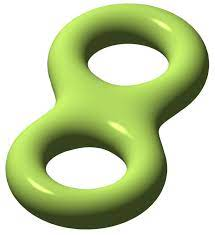
\includegraphics[scale=0.25]{genus-two}
\caption{The two holed torus (surface of genus of 2)}
\label{fig:genus-two}
\end{center}
\end{figure}

$$
\begin{pmatrix}
\text{Topological } \\
\text{spaces}
\end{pmatrix}
\bigleadsto
\begin{pmatrix}
\text{Quantum\,} \\ \text{systems}
\end{pmatrix}.
$$

All of the interesting quantum systems are in two dimensional spaces. This can be seen as follows. TQC is performed by braiding quasiparticles through spacetime. When space is two dimensional, spacetime is three dimensional. When space is three dimensional, spacetime is four dimensional. It is a theorem that there are no knots in four dimensions: The extra dimension gives the knot room to move around and untangle. Thus, to have nontrivial knots, space must be two dimensional. A two dimensional space is called a \textit{surface}. The surfaces we are interested in are those two dimensional spaces which can be embedded into three dimensional space, i.e., those surfaces which can be realized physically in our three dimensional world. Note that there are some weird surfaces which can not be embedded into three dimensional space, such as the Klein bottle (shown in Figure  \ref{fig:klein-bottle}). While the `true' surface does not intersect itself, any way of placing it in three dimensions will self intersect. One needs an extra dimension to avoid this intersection.

\begin{figure}
\begin{center}
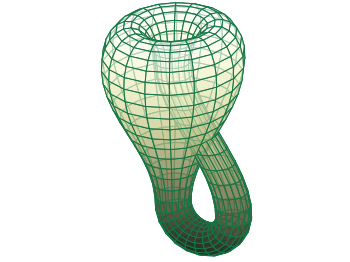
\includegraphics[scale=0.25]{klein-bottle}
\caption{The Klein bottle, attempting to be embedded in 3d space}
\label{fig:klein-bottle}
\end{center}
\end{figure}

This condition on embeddability into three dimensional space makes our study of surfaces much simpler. Namely we have the following well-known theorem from topology:

\begin{theorem} Consider a surface that

\begin{enumerate}
\item Is finite in area (for example, an infinitely stretched flat plane would not count)
\item Has no boundary (for example, a unit disk would not count, since its boundary is the circle)
\item  Can be embedded into three dimensional space.
\end{enumerate}

Then, this surface must be a collection of $g$-holed torii, for some integers $g\geq 0$.
\end{theorem}

Thus, going forward the word `surface' will simply refer to a collection of $g$-holed torii. A connected surface is one which can not be decomposed as the union of two other smaller surfaces. Every connected surface will be the $g$-holed torus for some $g\geq0$, and more general surfaces can all be uniquely written as a union of connected surfaces. A two dimensional topological quantum phase of matter is thus an assignment

$$
\begin{pmatrix}
\text{Surfaces} \\
\text{in space}
\end{pmatrix}
\bigleadsto
\begin{pmatrix}
\text{Quantum\,} \\ \text{systems}
\end{pmatrix}.
$$

Mathematically, a quantum system is a complex vector space. Hence, a topological quantum phase of matter is an assignment

$$S \,\mathlarger{\leadsto}\,V(S),$$

where $S$ is a surface and $V(S)$ is a finite dimensional vector space over the complex numbers. This mathematical formalism is known as Topological Quantum Field Theory. Namely, the assignment $S \,\mathlarger{\leadsto}\,V(S)$ \textit{is} a Topological Quantum Field Theory. To ease terminology, we will from now on use the acronym TQFT.

Not every assignment of surfaces to vector spaces will be a TQFT. Namely, many will be `un physical', meaning that they never could have come from topological phases of matter. For example, the axioms of quantum mechanics say that putting two quantum systems together should correspond to the tensor product of those systems. Formally, we should have

$$V\left(S_0\sqcup S_1\right)=V(S_0)\otimes V(S_1).$$

Here, $\sqcup$ denotes the disjoint union. The disjoint union is the same as a union, but it specifies that the union should be taken in a way such that $S_0$ and $S_1$ do not intersect (i.e. that they are disjoint). The disjoint union can be intuitively read as simply putting two spaces next to each other.

Additionally, by the axioms of quantum mechanics, transformations of a surface through spacetime should correspond to linear maps on quantum systems. We think mathematically about what a trajectory through spacetime looks like. In the one dimensional case, suppose we have two particles $a$ and $b$. A trajectory through spacetime from $a$ to $b$ is a path $e$ connecting $a$ and $b$. Thinking deeply, one observes that the condition of ``connecting" $a$ and $b$ can be mathematically stated as $\partial e= a \sqcup b$, where $\partial e$ denotes the boundary of $e$. This is shown in Figure \ref{fig:bordism}.

\begin{figure}
\begin{center}
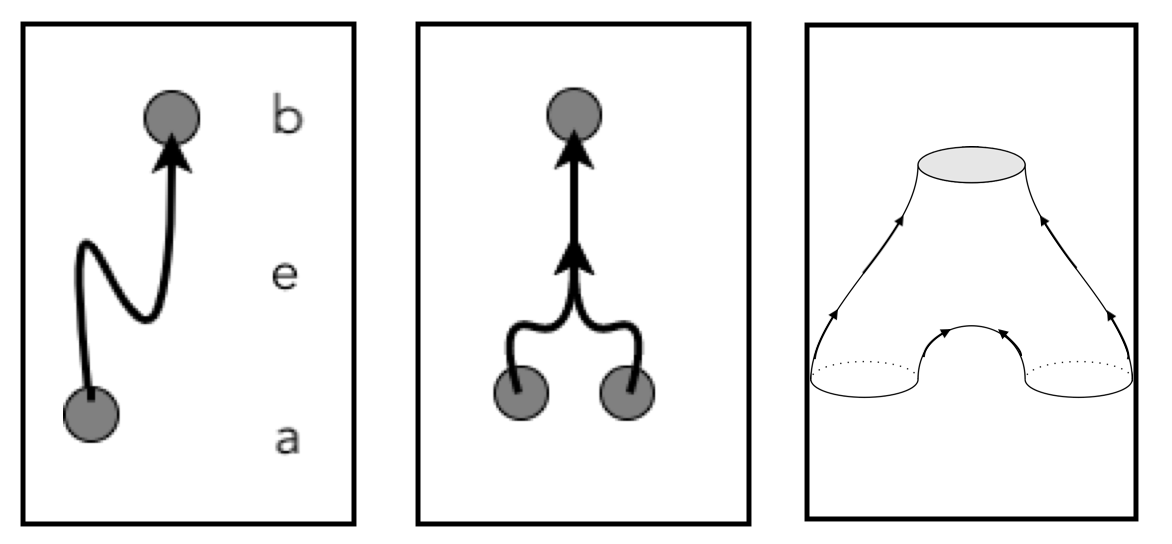
\includegraphics[scale=0.40]{cobordism}
\caption{First box - A path in spacetime from $a$ to $b$ by $e$, i.e., a path $e$ with $\partial e= a \sqcup b$. Second box - The fusion of two particles in spacetime. Third box - the fusion of two circles in spacetime, known informally as a ``Pair of Pants".}
\label{fig:bordism}
\end{center}
\end{figure}

We observe however an ambiguity: Time has direction, but our edge a-priori does not. Hence, it is impossible to distinguish a path from $a$ to $b$ and a path from $b$ to $a$. For this reason we have to introduce the concept of \textit{orientation}. An oriented path is a path with a choice of direction. This can be visualized by putting a consistent set of arrows on the path. The points at the back end of the arrow correspond to the particles at the start of the process, and the points at the front end of the arrow correspond to the particles at the end of the process. Note that the paths can join and split, as seen in the second box of Figure  \ref{fig:bordism}. This corresponds to the fusion and annihilation of particles.

Working one dimension higher, we can imagine the trajectory of circles of particles - loops - through spacetime. The merging of two circles will look exactly like it did before, except that now instead of tracing a path through spacetime it will trace a surface with boundary. The boundary components correspond exactly to the particles at the start and end of the process, as seen in the third box of Figure \ref{fig:bordism}.

We now try to generalize this picture to the case of surfaces. Remember, our goal is to mathematically describe a trajectory of surfaces through spacetime, which will be key to our theory since these will correspond to linear transformations on quantum systems. The key insight is as follows. Given two sets of $A$ and $B$ (still representing particles), we saw a trajectory through spacetime was a path $E$ such that $\partial E=A\sqcup B$. Given two collections of circles $A$ and $B$, we saw a trajectory through spacetime was a surface $E$ such that $\partial E=A\sqcup B$. Given two surfaces $S_0$ and $S_1$ (with no boundary, as usual), a trajectory through spacetime should be a three dimensional object $X$ whose boundary is $\partial X= S_0\sqcup S_1$.

Defining what we mean exactly by three dimensional object is very technical. Namely, these objects should be $3$-manifolds, in the same way that a surface is a $2$-manifold, a path is a $1$-manifold, and a set of points is a $0$-manifold. An introduction to the theory of manifolds can be found in Spivak's textbook \cite{spivak2018calculus}. We leave the notion vague. One can think of 3-manifolds as being filled in surfaces. For instance, the torus is a surface ($2$-manifold), but the filled in solid torus is a $3$-manifold. Let $X$ be the solid torus with a smaller solid torus removed from inside it. Then the boundary $\partial X$ will be equal to the disjoint union of the outside torus and the smaller inside torus. We can see that $X$ forms a trajectory through spacetime, as the bigger torus contracts onto the smaller one. There is still one ambiguity. How do we know that $X$ is a contraction big to small? Instead, it could have been an expansion small to big. To fix this issue we will again have to speak of oriented $3$-manifolds. Oriented manifolds are (loosely) manifolds with a coherent system of arrows giving direction at every point. For example, a series of arrows in $X$ all pointing from the big outside torus toward the smaller inside torus is an orientation.

We introduce a piece of notation. When $\partial X = S_0 \sqcup S_1$ is the disjoint union of two surfaces, one of those surfaces (say, $S_0$) will always be the stuff going in, and one of those surfaces (say, $S_1$) will always be the stuff going out. We call this a \textit{bordism}\footnote{Sometimes called a cobordism; the difference is immaterial.} from $S_0$ to $S_1$. Namely, a bordism from a surface $S_0$ to a surface $S_1$ is an oriented $3$-manifold $X$ such that $\partial X = S_0\sqcup S_1$, where all of the arrows in the orientation of $X$ are pointing away from $S_0$ and towards $S_1$ . With this out of the way, we can formally define a TQFT:

\begin{definition}[$(2+1)$-TQFT] A $(2+1)$ Topological Quantum Field Theory (TQFT) is the following data.
\begin{enumerate}
\item A choice of finite dimensional complex vector space $V(S)$ for every surface $S$.
\item A choice of linear transformation $Z(X): S_0\xrightarrow{} S_1$ for every bordism $X$ from $S_0$ to $S_1$.
\end{enumerate}
Additionally, a $(2+1)$-TQFT is required to satisfy the following properties:
\begin{enumerate}

\item (Union = tensor product). $V(S_0\sqcup S_1)=V(S_0)\otimes V(S_1)$. Here, $S_0$ and $S_1$ are any two surfaces.

\item (Do nothing = identity) $Z(S\times [0,1])=\text{id}_{V(S)}$. Here, $S\times [0,1]$ is the Cartesian product of $S$ with the interval, treated as a bordism from $S$ to itself. Concretely $\partial (S\times [0,1])=S\times\{0\}\sqcup S\times\{1\}$, and we identify $S\times \{0\}$ and $S\times\{1\}$ both with $S$.

\item (Composing bordisms = composing maps). $Z(X_1\cup X_0)=Z(X_1)\circ Z(X_0)$. Here, $X_0$ is a bordism from two surfaces $S_0$ and $S_1$ and $X_1$ is a bordism from surfaces $S_1$ to $S_2$. One easily verifies that their union $X_1\cup X_0$ is a bordism between $S_0$ and $S_2$, whose induced map we can compare with the composition of the induced maps of $X_0$ and $X_1$.

\item (Swap spaces = swap tensor factors) $Z(X)(v_0\otimes v_1)=v_1\otimes v_0$ for all $v_0\in V(S_0)$, $v_1\in V(S_1)$. Here, $X$ is the bordism from $S_0\sqcup S_1$ to $S_1\sqcup S_0$ defined by taking $S_0,S_1$ and moving them around each other.
\end{enumerate}

\end{definition}

We offer a few remarks. The term ``$(2+1)$" refers to the fact that there are two space dimensions, plus one time dimension. More generally, an  $(n+1)$-TQFT is an assignment of $n$-manifolds to vector spaces, and of $(n+1)$-manifolds to linear transformations. We also remark on the structure of the definition. We first defined a few assignments of objects of one type to objects of another type, and then we defined a laundry list of properties that those assignments should satisfy. This is extremely standard practice in higher mathematics. The abstraction of this practice is known as Category Theory. The assignments of one type of object to another type of object are known as functors, and the properties to satisfy are known as axioms. The category theory definition of a TQFT is ``a symmetric monoidal functor from the category of bordisms to the category of vector spaces"\footnote{symmetric=axiom 4, monoidal=axiom 1, functor=axiom 3, bordsism category=axiom 2}. For those unfamiliar with category theory, a short introduction is found in Appendix \ref{Categories}. While we will not be using any categories in this section, a familiarity of the subject is required for the following section on Modular Tensor Categories.

Often, TQFTs will be defined in terms of celluations. A celluation is a way of splitting up a space into vertices, edges, and faces. The utility of celluations is that they turn continuous objects into discrete ones, which allows for simple computations - this was the entire point of modeling the torus as an $n$ by $n$ grid in Section \ref{The Toric Code}. The difficult part is often showing that the object you defined is independent of the choice of celluation. For the toric code, this was Exercise \ref{The Toric Code}.3. In general, one resorts to the following theorem:

\begin{theorem}[Pachner, \cite{pachner1991pl}, \cite{lickorish1999simplicial}]\label{Pachner} Let $(X,\Delta_X)$ and $(X,\Delta'_X)$ be two manifolds with triangulations (i.e. celluations in which every face has three edges). There exists a finite sequence of so-called Pachner moves relating $\Delta_X$ to $\Delta'_X$. In two dimensions (i.e. when $X$ is a surface) and three dimensions, the full list of Pachner moves is given in Figure \ref{fig:all-moves}. The naming convention is that the ``$a$-$b$" move is the move that takes $a$ cells to $b$ cells.
\end{theorem}

\begin{figure}
\begin{center}
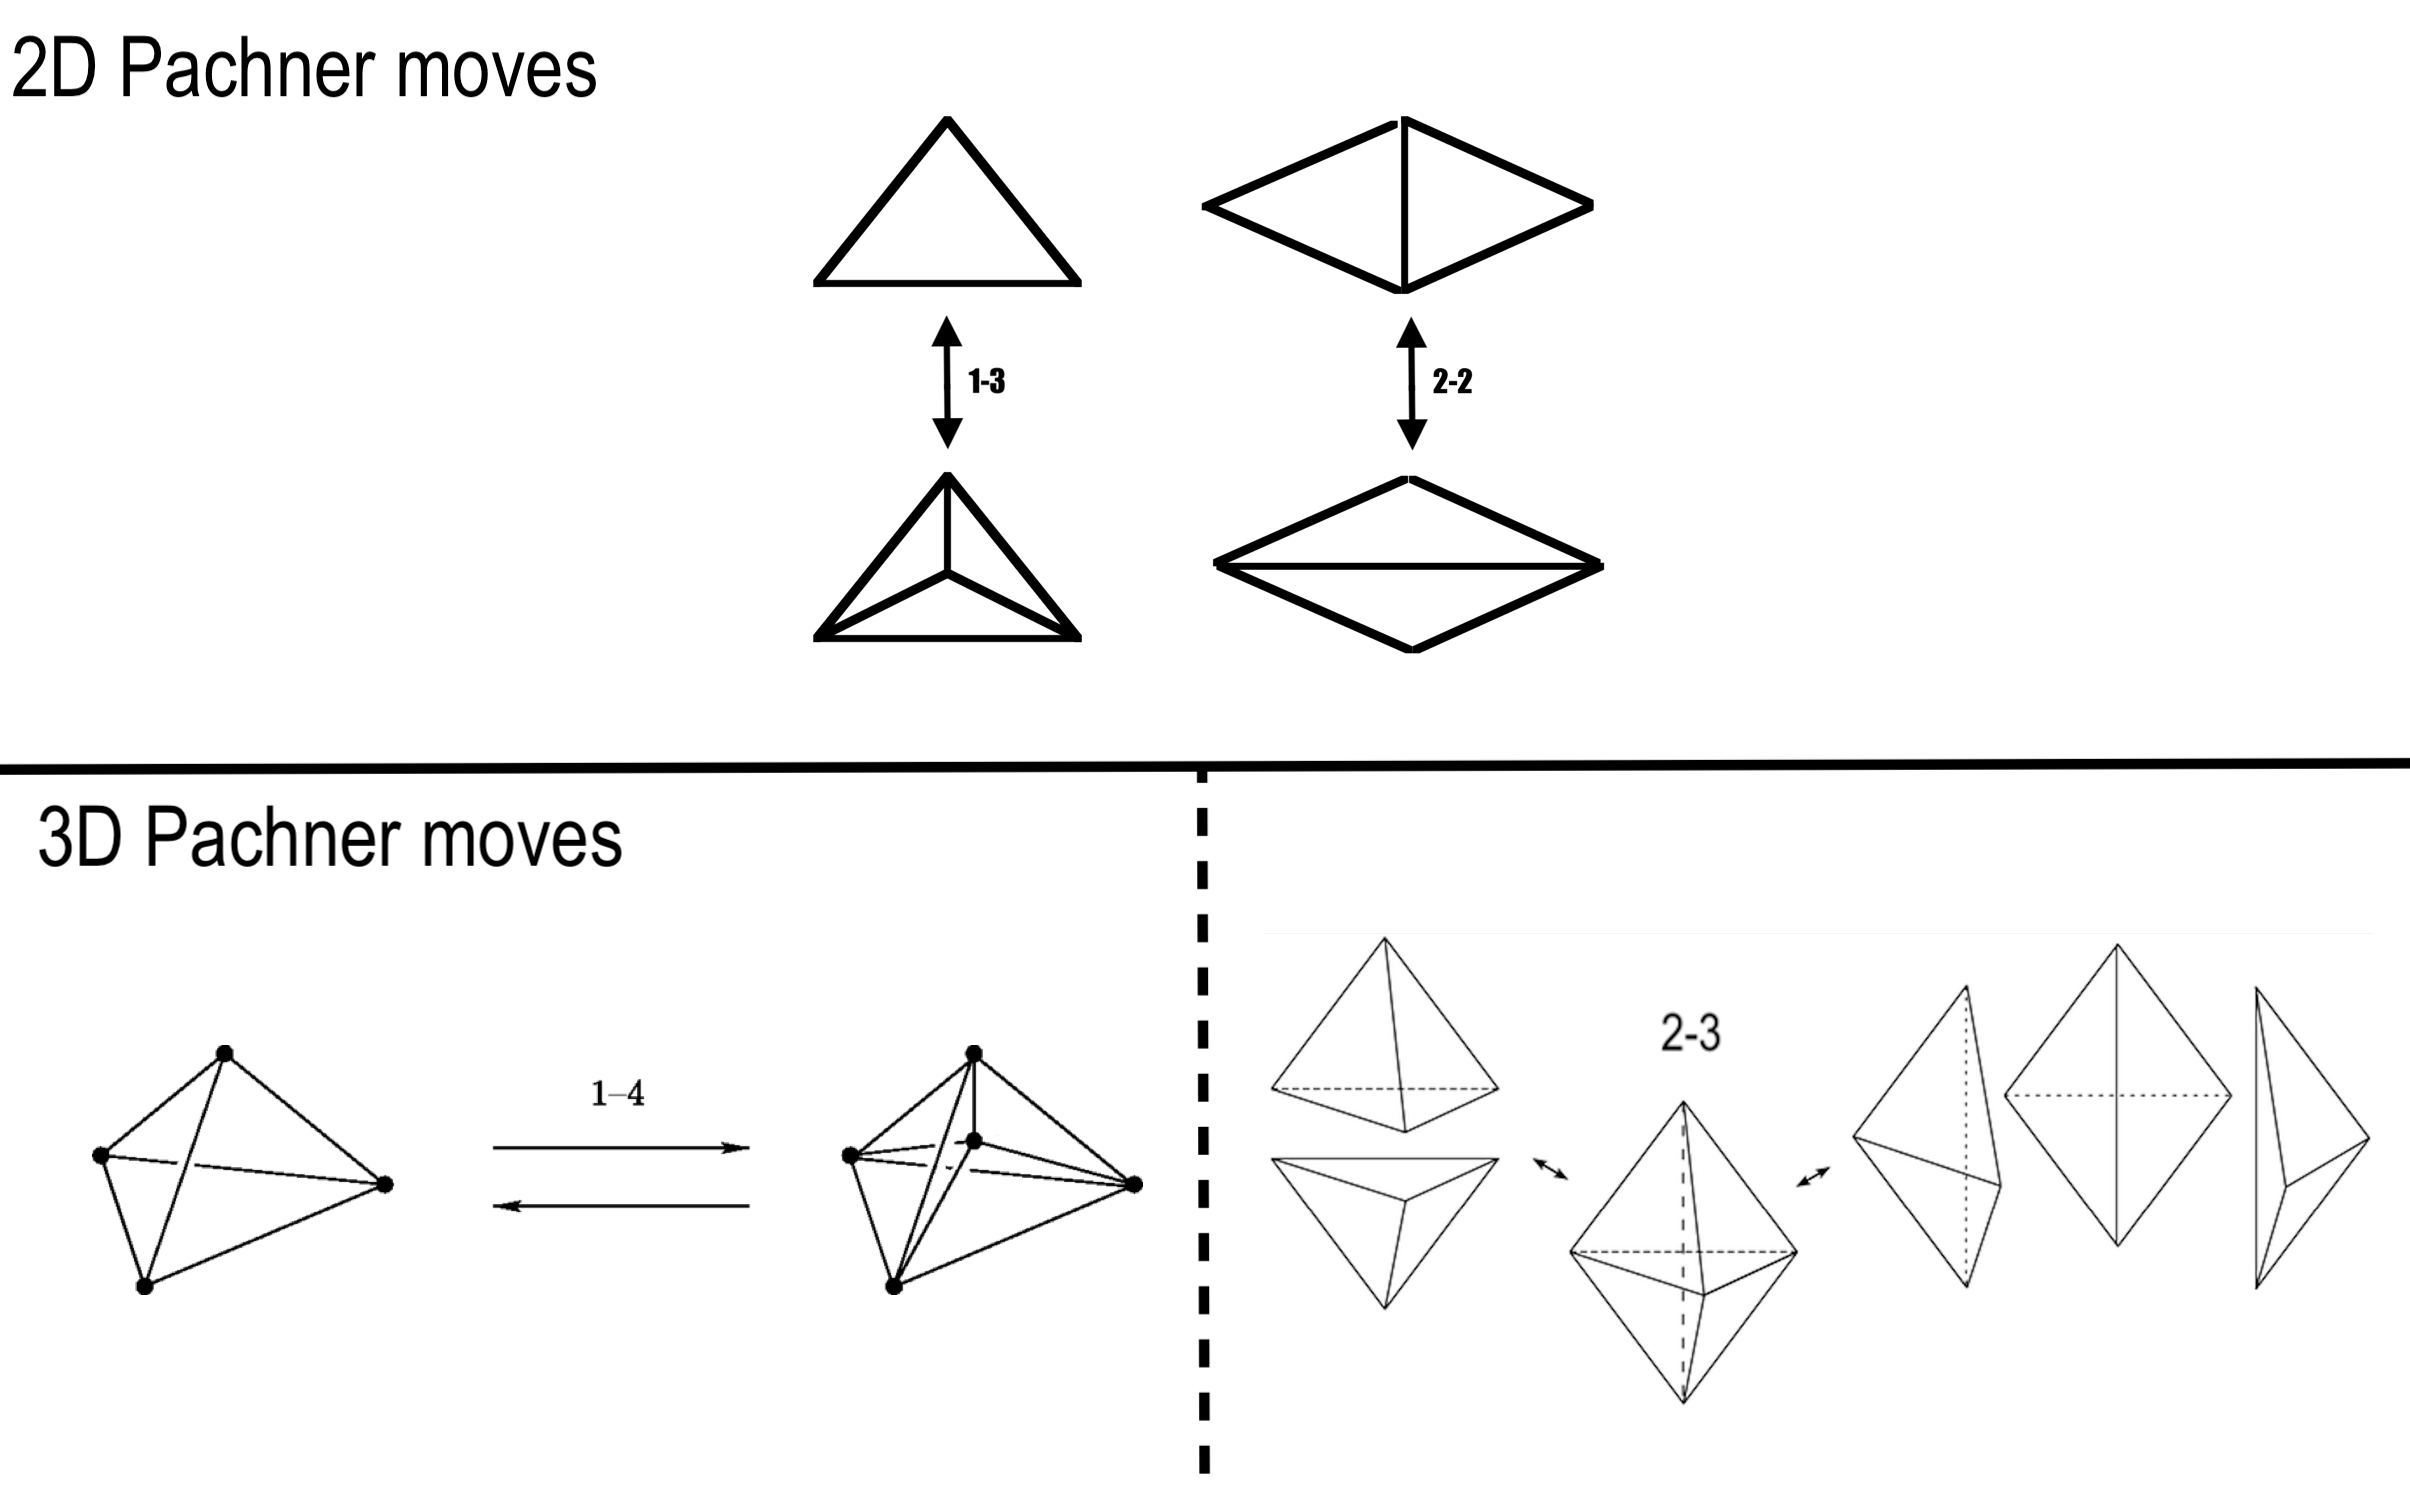
\includegraphics[scale=0.2]{all-moves}
\caption{The Pachner moves.}
\label{fig:all-moves}
\end{center}
\end{figure}


This massively facilitates the verification of whether or not a definition is independent of celluation. Namely, first you show that the definition is invariant under adding/removing edges (allowing you to turn the celluation into a triangulation), and then you check that the definition is invariant under applying the Pachner moves. Typically, this verification is entirely elementary and does not require any great show of cleverness. As such, our standard practice for  Subsection \ref{DW TQFT} will be to state theorems, reduce the problem to the verification of invariance under Pachner moves, and assign the rest as an exercise to the reader.

\subsection{The $\ZZ_2$ Dijkgraaf-Witten TQFT}
\label{DW TQFT}

We now define the Topological Quantum Field Theory (TQFT) associated with the toric code, and describe how TQC can be performed in this framework. We could also call it the ``$\ZZ_2$ spin liquid TQFT", since it is the mathematical realization of the $\ZZ_2$ spin liquid topological quantum phase of matter. The original reference for this subject is \cite{dijkgraaf1990topological}, but our presentation follows more closely \cite{qiu2021representations}.

As with the definition of the toric codes in Section \ref{The Toric Code}, the definition of the $\ZZ_2$ Dijkgraaf-Witten TQFT is in the language of $\ZZ_2$ homology. Seeing as our definition of homology requires a celluation we first define $\tilde{V}(S,\Delta)$, where $S$ is a surface and $\Delta_S$ is a celluation of $S$. That is, $\Delta_S$ is a representation of $S$ as a collection of vertices, edges, and faces, with some edges and vertices identified. For example, $S=T$ could be the torus, and $\Delta$ could be the $n$ by $n$ lattice with opposite edges identified. For every surface $S$ and celluation $\Delta_S$, we define

$$\tilde{V}(S,\Delta_S)=\CC\left[C^{1}(\Delta_S;\ZZ_2)\right].$$

Here $C^1(\Delta_S;\ZZ_2)$ denotes the group $\ZZ_2$ cocycles on the celluation $\Delta_S$, and $\CC[-]$ is notation for ``complex vector space generated by", i.e., $\tilde{V}(S)$ is the unique complex vector space having $C^1(\Delta_S;\ZZ_2)$ as a basis. A $\ZZ_2$ cocycle is an assignment of $0$s and $1$s to every edge, such that every face touches an even number of $1$-labeled edges.

Notice that a $\ZZ_2$ cocycle is the same thing as a $\ZZ_2$ cycle in the dual celluation, as discussed in the proof of Proposition \ref{Xparticle}. That is, every $\ZZ_2$ cocycle on $S$ specifies a cycle on $S$, by drawing lines between the centers of two faces whenever the edge connecting them is labeled by a $1$. This process of identifying cocycles on $\Delta_S$ and cycle in the dual celluation is known as Poincaré Duality. It is important to note that in higher dimensions the process breaks down, because generically loops will fail to intersect in three dimensions (they can just be shifted past each other). Thus, when discussing 3-manifold bordisms there is a real distinction between cycles and cocycles.

The reason we call this $\tilde{V}$ instead of $V$ is that it depends on the choice of celluation $\Delta_S$, and we want $V(S)$ to only depend on $S$. The invariant subspace $V(S)$ is defined like so:

$$V(S)=\CC[H^1(S;\ZZ_2)],$$

where $H^1(S;\ZZ_2)$ is the cohomology of $S$. Cohomology is defined by

$$H^1(S;\ZZ_2)=C^1(S;\ZZ_2)/Z^1(S;\ZZ_2),$$

where $Z^1(S;\ZZ_2)$ is the subgroup of $C^1(S;\ZZ_2)$ generated by the cocycles consisting of $1$s at every edge touching a vertex. Assigning $1$s and $0$s this way really does give a cocycle: Every face has either $0$ or $2$ edges in its boundary that touch a given vertex, and both $0$ and $2$ are even numbers. It is a standard fact that the cohomology of a space does not depend on the choice of celluation.

To view $V(S)$ and a subspace of $\tilde{V}(S,\Delta_S)$, we define a linear injection

\begin{align*}
V(S)&\hookrightarrow \tilde{V}(S,\Delta_S).\\
\left|\alpha\right>&\mapsto \frac{1}{\sqrt{|Z^1(S;\ZZ_2)|}}\sum_{\gamma\sim \alpha}\left|\gamma\right>
\end{align*}

Here, $\alpha$ is a cohomology class (an element of $H^1(S;\ZZ_2)$), $\left|\alpha\right>$ is the corresponding vector in $V(S)$, $|Z^1(S;\ZZ_2)|$ denotes the number of elements in $Z^1(S;\ZZ_2)$, and $\sim$ denotes the equivalence relation of being cohomologous. That is, two cocycles are cohomologous if they give the same element in $H^1(S;\ZZ_2)$. This map can be summarized by saying that a cohomology class sends to the equal superposition of all of its representatives. The normalizing factor $|Z^1(S;\ZZ_2)|^{-1/2}$ is introduced to make sure that the norm is preserved.

We now define the action of bordisms. Let $(S_0,\Delta_{S_0})$ and $(S_1,\Delta_{S_1})$ be two surfaces with celluations. Let $X$ be a bordism from $S_0$ to $S_1$. Let $\Delta_X$ be a celluation on $X$ compatible with the celluations on $S_0$ and $S_1$. By compatible we mean that if we restrict $\Delta_X$ to $\partial X$ then we will recover the celluations $\Delta_{S_0}$ and $\Delta_{S_1}$. This restriction process can be described visually as dropping all verticies, edges, and faces, from $\Delta_X$ that aren't part of $\partial X=S_0\sqcup S_1$. We call a pair of cocycles $(\omega_{S_0},\omega_{S_1})$ extendable if there is a cocycle in $\omega_X\in C^1(X,\Delta_X)$ which gives $\omega_{S_0}$ when restricted to $S_0$ and $\omega_{S_1}$ when restricted to $S_1$. Let $N_X$ be the number of cocycles in $C^1(S_1;\ZZ_2)$ with which the $0$ cocycle on $S_0$ can be extended. We define

$$\tilde{Z}(X,\Delta_X)=\frac{1}{N_X}\begin{pmatrix}
$1$\text{ if }(\omega_{S_0},\omega_{S_1})\text{ extendable}\\
$0$\text{ otherwise }
\end{pmatrix}_{\substack{\omega_{S_0}\in C^1(S_0;\ZZ_2) \\ \omega_{S_1}\in C^1(S_1;\ZZ_2)}}.$$

We now elaborate on the meaning of this expression. Linear algebra tells us that to specify a linear transformation between two spaces, all we need to do is specify the entries of a matrix. The entries of a matrix are labeled by basis vectors. Namely, the matrix entries of a map from $\CC[C^1(S_0;\ZZ_2)]$ to $\CC[C^1(S_1;\ZZ_2)]$ are labeled by ordered pairs of basis vectors $(\left|\omega_{S_0}\right>,\left|\omega_{S_1}\right>)$, where $\omega_{S_0}\in C^1(S_0;\ZZ_2)$ and $\omega_{S_1}\in C^1(S_1;\ZZ_2)$. The $(\left|\omega_{S_0}\right>,\left|\omega_{S_1}\right>)$ entry in $\tilde{Z}(X;\Delta_X)$ is equal to $1$ if $(\omega_{S_0},\omega_{S_1})$ is extendable, and $0$ otherwise.

The intuition for $\tilde{Z}(X,\Delta_X)$ comes from the path integral formulation of quantum mechanics. When not being observed, a system will transform along an equal superposition of all possible trajectories. There is a spacetime trajectory sending a state (cocycle) $\left|\omega_{S_0}\right>$ to a state (cocycle) $\left|\omega_{S_1}\right>$ exactly when $(\omega_{S_0},\omega_{S_1})$ can be extended. The map $\tilde{Z}(X,\Delta_X)$ can be described as the transformation that takes a state to the equal superposition of all possible states it could go to.

Our goal is to show that $\tilde{Z}(X,\Delta_{X})$ restricts to a map $V(S_0)\xrightarrow{}V(S_1)$, and that this restriction is independent of our choice of $\Delta_{S_0}, \Delta_{S_1}$ and $\Delta_{X}$. Once this has been done we can define $Z(X)$ to be this common restriction. All that will be left to do then is to show that our assignments $V(S)$ and $Z(X)$ satisfy the axioms of a $(2+1)$-TQFT. We work on this overarching plan over the course of a few propositions.

\begin{proposition}\label{Celluation independent}
Let $(S_0,\Delta_{S_0})$ and $\left(S_1,\Delta_{S_1}\right)$ be surfaces with celluations, $X$ a bordism from $S_0$ to $S_1$, and $\Delta_X$ a celluation of $X$ compatible with the celluations on $S_0$ and $S_1$. Then, the map $\tilde{Z}(X,\Delta_X): \tilde{V}(S_0,\Delta_{S_0})\xrightarrow{}\tilde{V}(S_1,\Delta_{S_1})$ is independent of the choice of celluation $\Delta_X$. Hence, we can properly omit $\Delta_X$ from our notation, and speak of a well defined map $\tilde{Z}(X)$.
\end{proposition}
\begin{proof} We need to show that if $\Delta_X$ and $\Delta'_X$ are two different choices of celluations on $X$ compatible with $\Delta_{S_0}$ and $\Delta_{S_1}$, then then $\tilde{Z}(X,\Delta_X)=\tilde{Z}(X,\Delta'_X)$. That is, $(\omega_{S_0},\omega_{S_1})$ are extendable in $\Delta_X$ if and if they are extendable in $\Delta_X'$. By Theorem \ref{Pachner}, all we have to do is show that the property of $(\omega_{S_0},\omega_{S_1})$ being extendable is invariant first under the operation of adding/removing edges (to turn the celluation into a triangulation), and secondly invaraint under the process of applying Pachner moves. Drawing out the diagrams, these are straightforward computations. We leave the verification of the proof as an exercise to the reader (Exercise \ref{TQFTs}.1).
\end{proof}

\begin{lemma}\label{independence} Let $(S_0,\Delta_{S_0})$, $(S_1,\Delta_{S_1})$, $(S_1,\Delta_{S_2})$ be surfaces with celluations, let $X_0$ be a bordism from $S_0$ to $S_1$, and let $X_1$ be a bordism from $S_1$ to $S_2$.

\begin{enumerate}[(i)]
\item $|\left\{\omega_{S_1}\in C^1(\Delta_{S_1};\ZZ_2) \st (\omega_{S_0},\omega_{S_1}) \text{ extendable}\right\}|$ is independent of choice of $\omega_{S_0}$
\item $|\left\{\omega_{S_1}\in C^1(\Delta_{S_1};\ZZ_2)\st (\omega_{S_0},\omega_{S_1})\,\, \& \,\,(\omega_{S_1},\omega_{S_2})\text{ extendable}\right\}|$ is independent of choice of $\omega_{S_0}$, $\omega_{S_2}$, so long as $(\omega_{S_0},\omega_{S_2})$ is extendable
\end{enumerate}
\end{lemma}
\begin{proof} We prove $(i)$, and leave $(ii)$ as an exercise (Exercise $\thesection.2$) since the proof is identical. Let $\omega_{S_1}$ and $\omega_{S_1}$ be such that $(\omega_{S_0},\omega_{S_1})$ and $(\omega_{S_0},\omega'_{S_1})$ are extendable. Then, adding extensions of these pairs together edgewise we get that $(\omega_{S_0}+\omega_{S_0},\omega_{S_1}+\omega'_{S_1})$ is extendable. Since $\omega_{S_0}+\omega_{S_0}=0$, we find that there is a $1$-to-$1$ bijection between $\omega_{S_1}$ such that $(0,\omega_{S_1})$ is extendable and $\omega_{S_1}$ such that $(\omega_{S_0},\omega_{S_1})$ is extendable, sending $\omega_{S_1}$ to $\omega_{S_0}+\omega_{S_1}$ Thus, these sets have the same cardinality, and we conclude $(i)$.
\end{proof}

\begin{proposition}\label{composition} Letting $X_0,X_1$ be as in Lemma \ref{independence}, the composition law

$$Z(X_1\cup X_0)=Z(X_1)\circ Z(X_0)$$

holds.
\end{proposition}
\begin{proof} Expanding by matrix multiplication, we find by the definition of $Z(X)$ that the coefficient of $(\omega_{S_0},\omega_{S_2})$ in $Z(X_1)\circ Z(X_0)$ is

$$\frac{1}{N_{X_0}N_{X_1}}\sum_{\omega_{S_1}}
\begin{pmatrix}
$1$\text{ if }(\omega_{S_0},\omega_{S_1})\text{ extendable}\\
$0$\text{ otherwise }
\end{pmatrix}
\begin{pmatrix}
$1$\text{ if }(\omega_{S_1},\omega_{S_2})\text{ extendable}\\
$0$\text{ otherwise }
\end{pmatrix}.$$

The coefficient of $(\omega_{S_0},\omega_{S_2})$ in $Z(X_1\cup X_0)$ is $N^{-1}_{X_1\cup X_0}$ if $(\omega_{S_0},\omega_{S_2})$ extendable, and $0$ otherwise. Multiplying through, we find the equality we are trying to prove is

$$N_{X_0\cup X_1} |\left\{\omega_{S_1}\st (\omega_{S_0},\omega_{S_1})\,\, \& \,\,(\omega_{S_1},\omega_{S_2})\text{ extendable}\right\}|=N_{X_0} N_{X_1}.$$

Fix $\omega_{S_0}$. We claim that both sides of the above expression are equal to the number of pairs $(\omega_{S_1},\omega_{S_2})$ such that $(\omega_{S_0},\omega_{S_1})$ and $(\omega_{S_1},\omega_{S_2})$ are simultaneously extendable. The left hand side computes this value by first counting the number of ways of choosing $\omega_{S_2}$ (i.e. $N_{X_0\cup X_1}$), and the by counting the number of ways of filling in $\omega_{S_1}$. The right hand side computes this value by first counting the number of ways of choosing $\omega_{S_1}$ (i.e. $N_{X_0}$) and then counting the number of ways of choosing $\omega_{S_2}$ (i.e. $N_{X_1}$). Note the implicit use of Lemma \ref{independence}, saying that all of these values are equal. This completes the proof.

\end{proof}

The next proposition has a strong physical meaning, and can be seen as motivation for the fact that $V(S)$ is a ground state space. Namely, let $(S,\Delta_S)$ be a surface with celluation and let $S\times [0,1]$ be the product of $S$ with the real interval of numbers between $0$ and $1$. That is, elements of $S\times [0,1]$ are pairs $(s,t)$ where $s\in S$ and $t\in [0,1]$. This is a $3$-manifold, and gives a bordism from $S$ to itself. Namely, $\partial (S\times [0,1])$ is built of the two components $S\times \{0\}$ and $S\times \{1\}$. The orientation on $S\times [0,1]$ is induced by the orienation on $[0,1]$. This can viewed as the identity bordism: $S$ is doing nothing as time increases from $0$ to $1$. The boundary components correspond to the placement of $S$ at time $0$ and $S$ at time $1$. When time passes on a system, we expect it to ambiently decrease in energy. Thus,  physically $Z(S\times [0,1])$ should act by the identity on ground states, and send higher energy states down to the ground state. This is exactly the statement that $Z(S\times [0,1])$ should be a projection from the full state space to the ground state space. The following proposition in this lens thus says that $V(S)$ are exactly the ground space: [WORK: move some of this up to the previous section.]

\begin{proposition}\label{Z formula} Let $(S,\Delta_S)$ be a surface with celluation. Viewing $S\times [0,1]$ as a bordism from $S$ to itself, we have that $\tilde{Z}(S\times [0,1])$ is a projection from $\tilde{V}(S,\Delta_S)$ to $V(S)$. Namely, the image of $\tilde{Z}(S\times [0,1])$ is $V(S)$, and $\tilde{Z}(S\times [0,1])$ acts by the identity on $V(S)$. Explicitly, $\tilde{Z}(S\times [0,1])$ is given by the map

$$\left| \omega\right>\mapsto \frac{1}{|Z^1(\Delta_{S};\ZZ_2)|}\sum_{\gamma \sim \omega}\left|\gamma\right>.$$

\end{proposition}
\begin{proof} Let $\omega_{S}$, $\omega'_{S}$ be two cocycles on $\Delta_{S}$. We show that $(\omega_{S},\omega_{S}')$ is extendable if and only if $\omega_{S}$ and $\omega_{S}'$ are cohomologous. Consider the celluation $\Delta_{S\times [0,1]}$ obtained by adding an edge connecting each vertex in $S\times\{0\}$ to the corresponding vertex in $S\times \{1\}$.

\begin{figure}
\begin{center}
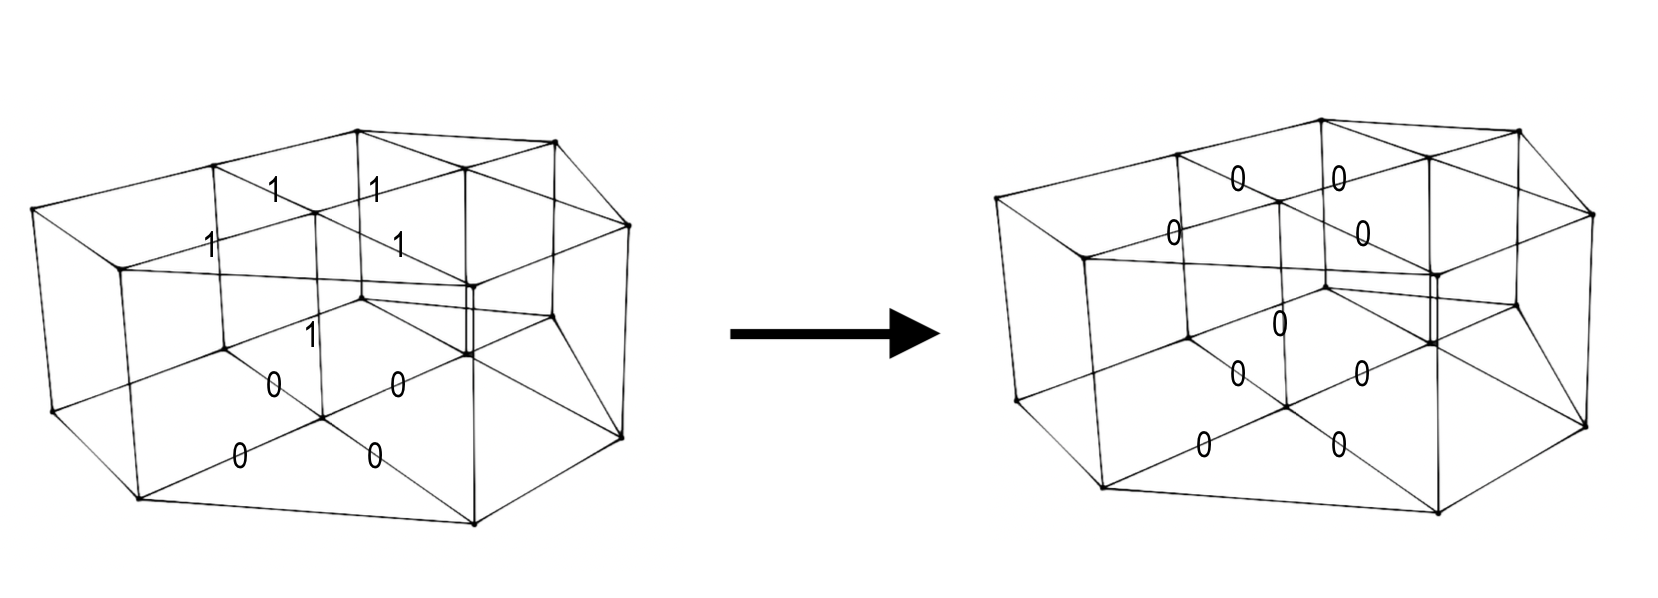
\includegraphics[scale=0.3]{cohomologous}
\caption{Removing the 1s from the central edges in $S\times [0,1]$}
\label{fig:cohomologous}
\end{center}
\end{figure}

We proceed by induction on the number of central edges in $S\times [0,1]$ (i.e. edges of $S\times [0,1]$ not in the boundary) which are assigned the value $1$ in the extension $\omega_X$ of $(\omega_{S},\omega_{S}')$. If there are no such edges, then clearly we must have $\omega_{S}=\omega_{S}'$, and so our proof is complete. Suppose there is a nonzero amount of such edges. Choose a central edge $e$ assigned $1$ in $\omega_X$. Let $\omega'_X$ the the cocycle obtained by flipping $e$ to as $0$, as well as flipping all of the edges touching $e$ in $S\times\{1\}$. $\omega'_X$ satisfies the cocycle condition since faces in the center touching $e$ will also touch exatly one of the edges flipped in $S\times \{1\}$, and hence the sum $1$s around the edges of those faces will change an even amount. By our inductive hypothesis, we conclude that $\omega_{S}'$ and $\omega_{S}$ are cohomologous. This process is demonstrated in Figure \ref{fig:cohomologous}.

The number of ways $N_{S\times [0,1]}$ of extending the $0$ cocycle is thus equal to the number of cocycles cohomologous to $0$, which is by definition $|Z^1(\Delta_S;\ZZ_2)|$. Thus, the stated formula is correct. It is straightforward to see that the rest of the proposition follows immediately from this formula.
\end{proof}

This allows us to prove the full independence of our theory from choice of celluation:

\begin{proposition}\label{S0S1 independence} Let $(S_0,\Delta_{S_0})$ and $\left(S_1,\Delta_{S_1}\right)$ be surfaces with celluations, and let $X$ be a bordism from $S_0$ to $S_1$. The image of $\tilde{Z}(X)$ is contained in $V(S_1)$. In particular, $\tilde{Z}$ restricts to a map $V(S_0)\xrightarrow{}V(S_1)$. This map is independent of our choice of $\Delta_{S_0}$ and $\Delta_{S_1}$. We define $Z(X): V(S_0)\xrightarrow{}V(S_1)$ to be this common restriction.
\end{proposition}
\begin{proof} To begin, we observe that if $(\omega_{S_0},\omega_{S_1})$ is extendable, then so is $(\omega'_{S_0},\omega_{S_1})$ for any $\omega'_{S_0}$ homologous to $\omega_{S_0}$. This follows by precomposing $X$ with $S_0\times [0,1]$, which does not change $X$, first extending $(\omega'_{S_0},\omega_{S_0})$ by Proposition \ref{Z formula}, and then extending $(\omega_{S_0},\omega_{S_1})$.

Thus, the equal superposition $\left|\omega_{S_0}\right>$ of every cocycle homologous to $\omega_{S_0}$ will map  under $\tilde{Z}(X,\Delta_X)$ to a sum of equal superpositions of cohomologous classes in $H^1(S_1;\ZZ_2)$, i.e., an element of $V(S_1)$. What is left to check is whether or not a cohomology class in $S_0$ can be lifted to a cohomology class in $S_1$ is independent of the choices of celluations.

To prove this, we consider the identity bordism $S\times [0,1]$ with $S\times \{0\}$ given a celluation $\Delta_{S}$ and $S\times \{1\}$ given a celluation $\Delta'_S$. We show that a cocycle in $C^1(\Delta_{S};\ZZ_2)$ can be lifted to a class in $C^1(\Delta'_{S};\ZZ_2)$ if and only if they are homologous. Applying this with $S=S_0$ and precomposing with $S_0\times [0,1]$ gives the desired independence of choice of celluation on $S_0$, and applying this with $S=S_1$ and postcomposing with $S_1\times [0,1]$ gives the desired independence of choice of celluation on $S_1$.

The above claim again follows from applying induction with respect to the moves in Theorem \ref{Pachner}, and thus is left as an exercise (Exercise $\thesection.3$).
\end{proof}

The main result of our section is as follows:

\begin{theorem} The assignments $S\mapsto V(S)$ and $X\mapsto Z(X)$ give a Topological Quantum Field Theory, called the $\ZZ_2$ Dijkgraaf-Witten TQFT.
\end{theorem}
\begin{proof} We check that our choices of $V(S)$ and $Z(X)$ satisfy the four axioms.

\begin{enumerate}
\item Specifying a cohomology class on $S_0\sqcup S_1$ amounts to specifying a cohomology class on $S_0$, and a cohomology class on $S_1$. In other words, we have a natural equality

$$H^1(S_0\sqcup S_1;\ZZ_2)=H^1(S_0;\ZZ_2)\times H^1(S_1;\ZZ_2).$$

Additionally, for any sets $A$ and $B$ we have $\CC[A\times B]=\CC[A]\otimes \CC[B]$, where we identity $[(a,b)]$ with $[a]\otimes [b]$, $a\in A$, $b\in B$. Thus,

\begin{align*}
V(S_0\sqcup S_1)&=\CC\left[H^1(S_0\sqcup S_1;\ZZ_2)\right]\\
&=\CC\left[H^1(S_0;\ZZ_2)\times H^1(S_1;\ZZ_2)\right]\\
&=\CC\left[H^1(S_1;\ZZ_2)\right]\otimes \CC\left[ H^1(S_1;\ZZ_2)\right]\\
&=V(S_0)\otimes V(S_1).
\end{align*}

\item This follows immediately from Proposition \ref{Z formula}.
\item This follows immediately from Proposition \ref{composition}.
\item The bordism $X$ has the effect of swapping $S_0$ and $S_1$, hence sends $H^1(S_0;\ZZ_2)\times H^1(S_1;\ZZ_2)$ to $H^1(S_1;\ZZ_2)\times H^1(S_0;\ZZ_2)$, sending $(\omega_{S_0},\omega_{S_1})$ to $(\omega_{S_1},\omega_{S_0})$. Tracing through the series of equalities in part 1, we get the desired result.
\end{enumerate}
\end{proof}

Seeing that the $\ZZ_2$ Dijkgraaf-Witten TQFT applied to the torus yields the toric code as defined in Section \ref{The Toric Code} is simple. The only difficulty comes from the fact that as defined, the toric code is generated by homology classes and the $\ZZ_2$ Dijkgraaf-Witten TQFT is generated by cohomology classes. However, as mentioned before, there is a duality between homology classes and cohomology classes which arises from considering the dual celluation, and so this discrepancy is really not an issue. We decided to work with homology in Section \ref{The Toric Code} for pedagogical reasons: homology is more intuitive than cohomology. However, for 3-manifolds there is a discrepancy between homology and cohomology, which is why the $\ZZ_2$ Dijkgraaf-Witten TQFT has to use the less intuitive concept.

In general, there is no Hamiltonian in TQFTs. The lowest energy states are those which will naturally occur after time passes, namely, those in the image of the ``do nothing" bordism $\tilde{Z}(X)$. It is for this reason that even though ground states are complicated maximally entangled objects (Exercise \ref{The Toric Code}.2) they are easy to make in the lab. All one has to do is make a cold enough system and allow it to relax. As time passes, it will naturally go into a ground state. In some quantum systems, these relaxed states are already interesting enough that it would take a long time to simulate the process on a classical computer. This gives a sort of quantum computer, known as an Adiabatic quantum computation. It is interesting to note that the original definition of the toric code did not include a Hamiltonian, and this was only introduced later to facilitate the study \cite{kitaev1997quantum}. A more general study of TQFTs with Hamiltonians was conducted by Levin-Wen \cite{levin2005string}, but is still not the norm.

In the TQFT language it is hard to see what anyons and quantum computations correspond to. How do I do braiding in a TQFT? How do I see how many particle types there are? The intriguing fact is that this information is present, but hidden. Namely, one has to pass to a \textit{1-extended TQFT} to engage with anyons explicitly. This extension allows us to define $V(S)$ whenever $S$ is a surface with punctures. These punctures correspond to anyons, and moving the punctures around each other corresponds to braiding. Not every TQFT can be 1-extended, but those that can (like the $\ZZ_2$ Dijkgraaf-Witten theory) keep that anyon information in their structure. A more complete introduction to TQC would have defined $1$-extensions, but we omitted the topic for clarity. All of this is in marked contrast to Modular Tensor Categories, where anyons are placed front and center of the theory.

$\newline\newline$

\large \textbf{Exercises}:\normalsize

\begin{enumerate}[\thesection .1.]
\item Complete the proof of Proposition \ref{Celluation independent}.

\item Complete the proof of Lemma \ref{independence}.

\item Complete the proof of Proposition \ref{S0S1 independence}.
\end{enumerate}

\section{Modular Tensor Categories}
\label{Modular Tensor Categories}

[WORK: Make section.]
\subsection{The data of an anyon model}
\label{Anyon model}

[WORK: Give the MTC description by label sets, fusion rules, and braiding relations. This should just be a big collection of numbers and some axioms they have to follow. Explain the physical concept that each set of numbers/relation corresponds to]

\subsection{The category-theoretic viewpoint}
\label{Category viewpoint}

[WORK: Give a bottom definition of Modular Tensor Category. State exactly how things correspond to the data of an anyon model. Main theorem: There could be multiple liftings to a category, maybe zero! Motivate category theory via commutative diagrams.]

\subsection{The MTC $\mathcal{Z}(\Vecc_{\ZZ_2})$}
\label{VecZ2 MTC}

[WORK: Define the MTC $\mathcal{Z}(\Vecc_{\ZZ_2})$ explicitly via data. Give a brief explanation of how this corresponds to the $\ZZ_2$ Dijkgraaf-Witten theory.Then, define $\Vecc_{\ZZ_2}$. State that the MTC defined is the Drinfeld center, to further motivate category theory. Analogy for Drinfeld center: (non-degenerate) abelianization. ]

\section{The Big Picture}
\label{The Big Picture}

[WORK: The big thing is to draw the picture between topological quantum phases of matter, TQFTs, MTCs, and TQC. Show exactly what this looks like in the case of the toric code, i.e., what the topological quantum phase of matter is, the TQFT, the MTC, and the resulting TQC. Add all the connections and insights that I've come up with along this journey, and things I would feel remiss not including. Really, this should be a version of an introduction-to-TQC-for-experts section. Should definitely mention that TQFTs are generally $1$-extended with punctures, to visualize anyons. Should mention that literally making torus bigger will make error rate smaller, since it's harder for things to accidentally interact with each other (exponential decrease). Maybe another thing to add is how the 1st priority is to minimize energy, and the 2nd order is to maximize entanglement.]

[WORK: Give 2nd motivation for topological quantum computing. Namely, that this might be a good avenue for proving that QC can solve NP complete problems, or close to NP problems! Bring up how this is clearly a good theory for computing knot invariants (add reference to examples of knot invariants that were proved to be easy to calculate using this method). Then, mention that computing the Jones polynomial is known to be NP hard! This is in the introduction of Wang and Rowell's ``Mathematics of Topological Quantum Computation". This could be a motivation for hybrid computing like

\begin{enumerate}
\item Use classical computers to reduce hard problems to the issue of finding the knot invariant of a given knot.
\item Create that knot by braiding the anyons through spacetime.
\item TQC will naturally compute the relevant knot invariant!
\end{enumerate}
]

\begin{quote}
``Folklore, [...] is a technical term for a method of publication in category theory. It means that someone sketched it on the back of an envelope, mimeographed it (whatever that means) and showed it to three people in a seminar in Chicago in 1973, except that the only evidence that we have of these events is a comment that was overheard in another seminar at Columbia in 1976. Nevertheless, if some younger person is so presumptuous as to write out a proper proof and attempt to publish it, they will get shot down in flames." - Paul Taylor \cite{aubert2019categories}
\end{quote}

[WORK: Here are some misc things for the rest of the manuscript.

In the introduction, maybe add something about the number of Nobel prizes associated with the area? Jones also got his fields medal for this stuff, and maybe others. Witten? Right at the end?

I got rid of the unit TQFT axiom, which now includes the degenerate possibility that $V(S)=\emptyset$ for all $S$. Is that okay?

Why can I always lift celluations? Zhenghan mentioned this in class, but didn't cite a reference.]
\appendix

\section{Quantum mechanics and quantum computation}
\label{Quantum mechanics}

[WORK: Introduce quantum mechanics for mathematicians. Really, this just means Von-Neumann axioms, a bit of quantum computing, and spectral theory.]

\section{$\ZZ_2$ Homology Theory}
\label{Homology}

In this appendix we introduce the basic notations of homology theory with $\ZZ_2$ coefficients, namely, chains, cycles, and homological equivalence. The settings for homology are \textit{simplicial complexes}, which can be loosely thought of as collections of vertices, edges, and faces, with some edges and vertices identified, just as was done for the torus in this text. A $\ZZ_2$-chain on a space is an assignment of an element of $\ZZ_2$ to every edge, where $\ZZ_2=\{0,1\}$ is the additive group modulo 2. The set of $\ZZ_2$-chains forms a group under edge-wise addition. A $\ZZ_2$-cycle is a $\ZZ_2$-chain which can be obtained by starting at a vertex and walking along edges, flipping $1$s to $0$s and vice versa as you go along, and returning back where you started at the end. Equivalently, a $\ZZ_2$-cycle is a $\ZZ_2$-chain which has an even number of $1$s touching each vertex. The $\ZZ_2$-cycles form a subgroup of the group of $\ZZ_2$-chains. Seeing as all chains and cycles discussed in these notes take coefficients in $\ZZ_2$, we ease notation by simply saying ``chain" and ``cycle".

The goal of homology theory is to describe cycles on a geometric object, up to deformations. If one cycle can be continuously deformed into another, then they should be considered equivalent. On the sphere, for example, all loops can be contracted away into nothing. On the torus there are four distinct cycles, namely, the zero cycle, the cycle that goes around the torus horizontally, the cycle that goes around the torus vertically, and the cycle that twists around the torus, as in Figure \ref{fig:homology} These non-trivial cycles correspond exactly to the continuous vector fields described in the introduction \cite{frankel1957homology}.

Loosely, we will call two cycles homologically equivalent if they can be continuously deformed one to another. Given any face, the cycle consisting of $1$s along the edges touching that face should be `homologically trivial", i.e., homologically equivalent to the $0$ cycle, since it can be contracted away into nothingness. In a strong sense, this is the only condition one needs to impose. WIth $X$ as our simplicial complex, we let $C_1(X;\ZZ_2)$ be the group of chains. We let $Z_1(X;\ZZ_2)$ be the subgroup generated by the cycles consisting of $1$s  the boundaries of faces. This is the subgroup of homologically trivial cycles. This lets us define the quotient

$$H_1(X;\ZZ_2)=C_1(X;\ZZ_2)/Z_1(X;\ZZ_2),$$

called the ($1$st) homology group of $X$. Two elements are called homologically equivalent if they are in the same coset of $H_1(X;\ZZ_2)$. Alternatively, two elements are homologically equivalent if one can be obtained from the other by repeatedly flipping $1$s and $0$s along the boundaries of squares.

It is a well known fact that the first homology group of the torus has four elements, corresponding to the zero class, the horizontal cycle around the torus, the vertical cycle around the torus, and the diagonal cycle.

The importance of $H_1(X;\ZZ_2)$ is that it is \textit{independent of choice of celluation}. Namely, if we start with the same space and chop it up into vertices, edges, and faces, two different ways, $H_1(X;\ZZ_2)$ will always be the same. This is in stark contrast to $C_1(X;\ZZ_2)$ and $Z_1(X;\ZZ_2)$, which will both change wildly depending on the choice of celluation.

The observant reader might find the above discussion frustrating. In particular, we seem to be using the following intuitions interchangeably:

\begin{enumerate}
\item Cycles being continuously deformed to each other
\item Cycles that can be obtained from one another by flipping edges along the boundary of faces.
\end{enumerate}

The worry regarding the distinction between these two notions is justified. In general, the group obtained by imposing the equivalence relation of continuous deformations will not be equal to the homology group $H_1(X)$. The group resulting from imposing the continuous deformation restriction is called the \textit{fundamental group} of $X$, and is denoted $\pi_1(X)$. In general $\pi_1(X)$ can be quite a bit larger than $H_1(X)$, i.e., the equivalence relation can be weaker. The groups are always related by the fact that $H_1(X)$ is canonically isomorphic to the abelianization of $\pi_1(X)$, i.e., the maximal abelian quotient of $H_1(X)$. In the case that $\pi_1(X)$ is abelian (for example, when $X$ is a torus), this means that there is no distinction between these spaces, and one should not make any worry about the discrepancies in intuition.

The canonical reference for this subject (known as \textit{Algebraic Topology}) is Alan Hatcher's textbook \cite{hatcher2005algebraic}.

\section{Category Theory}
\label{Categories}
[WORK: Make appendix. This is to mension for sure; canonical isomorphism between double duals, non canonical isomorphism between first duals. Not only is this super relevant to rigidity, but Zhenghan said that this was one of Eilenberg-MacLane's key motivations. Find a reference to this fact.]


\bibliographystyle{alpha}
\bibliography{ref}


\end{document}






